\chapter{Parallel and super scalar processors}

Recalling the previously seen formula:
$$T_{exec}=N_{instr}T_{clk} CPI$$

In ideal pipeline organization $CPI$ is equal to 1, however because of hazards (stalls, wrong branch prediction, etc.) this quantity will never reach one. In order to reduce the execution time there are two elements on which we can play: one is $T_{clk}$ (reducing critical path length), the other is $CPI$. Starting from a MIPS architecture, the choice of which parameter tuning leads to two different architectures:
\begin{itemize}
  \item Reducing $T_{clk}$ implies having a number of pipeline stages $m$ greater than 5, leading to \textbf{super-pipelined processor}. We cannot exaggerate with $m$ otherwise when the pipeline has to been discarded a lot of partially instructions are wasted. Moreover increasing $f_{clk}$ also power will increase, so this solution is not very good for low power processor.

  \item Having a CPI lower than 1, leading to \textbf{parallel processor}. There are two approaches to obtain a parallel process:
    \subitem Superscalar processors.
    \subitem VLIW processors.

\end{itemize}

In last two cases datapath is paralleled, there are several arithmetic units working in parallel and performing more than one instruction at the same time. In this case each datapath is still pipelined, so actually pipeline and parallel approaches are merged together.\\
In super-scalar processor nothing has to be done at compiler level since it is fully responsibly of process architecture recognize the parallel instructions, organized them and execute in parallel. So for the compiler point of view nothing changes because its output code is generated thinking that it will be executed sequentially.\\
In VLIW (Very Long Instruction Word) instead the processor takes from the compiler instructions which are already organized in parallel, no need to extract parallelism or check something. The difference is quite large, the second approach required much more capability for the compiler.

\section{Superscalar approach}
\begin{center}
  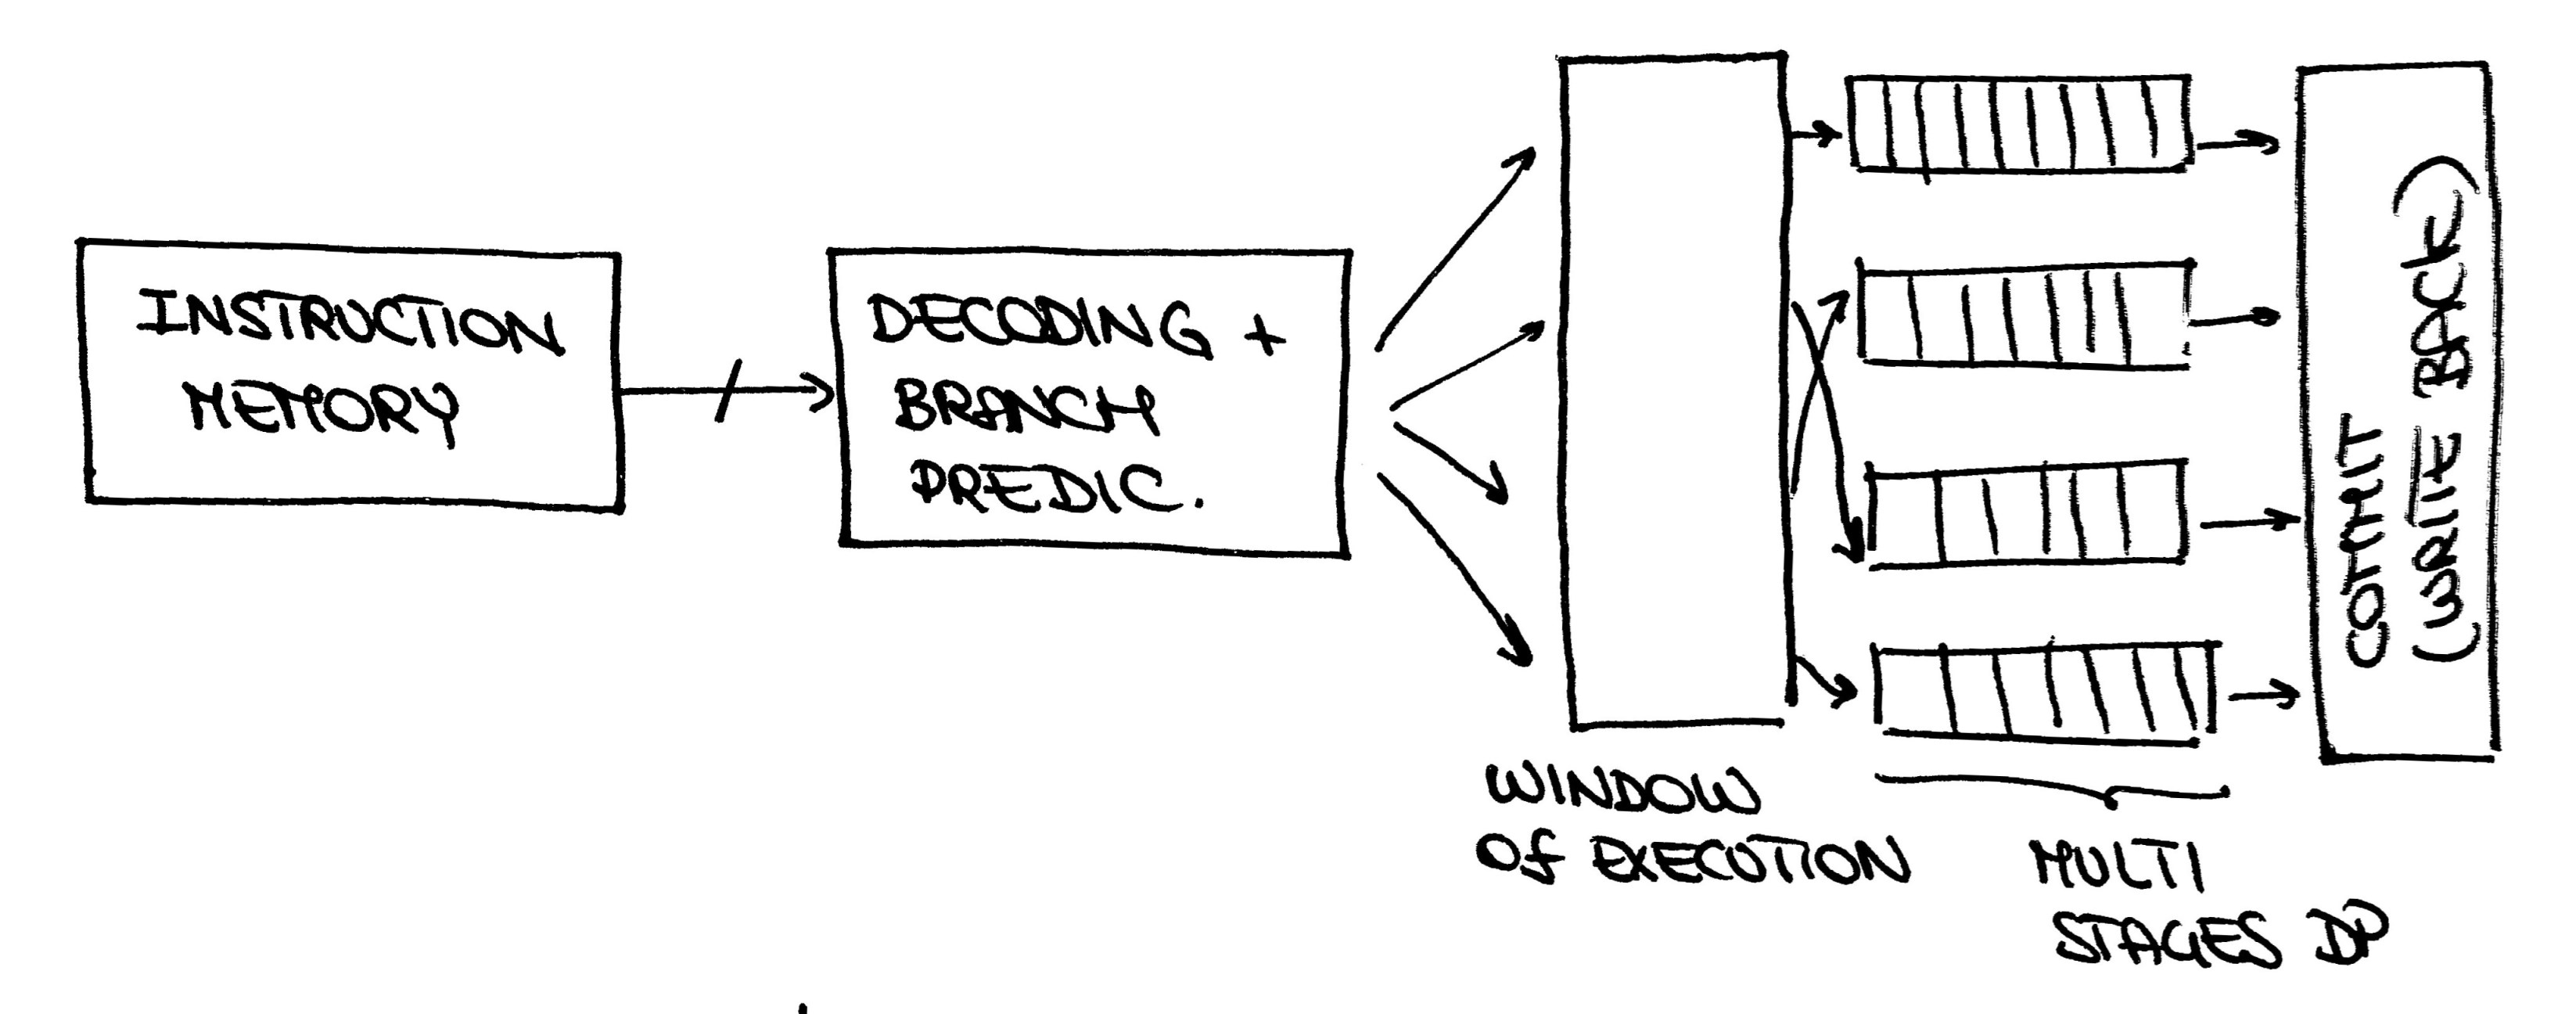
\includegraphics[width=0.7\linewidth]{img/img3/3}
\end{center}

We must be able to fetch more than one instruction from the memory, than in decoding stage there are more units than in MIPS, the most important one is the branch prediction. All instructions to be performed in parallel are stored in the so called window of execution, feed to datapaths (more than one stages) and finally reach the commit stage. It may happen that two instructions started at the same time (like an add and a div) reach the commit stage (where the result can be finally stored) in different time, meaning that there is the risk of writing the addition result before the division one: this may be a problem due to the fact that it may change the semantic of the application. Commit unit has to reorganize results, recreate the original order and write them in the order intended by the programmer. The key point is that if we allocate more than one datapath, these have to be efficiently used, meaning that the processor must be able to extract all the potential parallelism

\subparagraph{Example: window of execution}

C-code:

\begin{verbatim}
for(i=0; i< last; i++) {
    if(a[i]>a[i+1]) {
        temp=a[i];
        a[i]=a[i+1];
        a[i+1]=temp;
        change++;
    }
}
\end{verbatim}
Which is translated into:

\begin{verbatim}







\end{verbatim}


The code is organized in \textbf{basic blocks}, which correspond to a sequence of assembler instructions having a single entry-point, only one exit-point and no branches inside.\\


Ideally we could take every block and try to execute instructions inside it in parallel, this is simple since there are no branches inside a basic block. If we limit our search for parallel execution inside the basic block, we are not able to exploit all possibilities of parallel datapaths since inside each basic block there are a lot of data dependencies (due to how we write the code). The alternative approach consists of having a larger window, so considering more instructions coming from different basic blocks the probability to have some of them to be performed in parallel will increase. Since instructions now come from different basic blocks, there may be branches, so the problem is to understand if they can be executed in parallel.\\

The possibility of performing some instructions coming from different basic block depends on the possibility to take a certain branch: we can understand if instructions can be performed in parallel only having a branch prediction unit telling us if a certain branch will be taken or not, so in this way we can understand if we can merge basic block 1+2 or 1+3. \\

The window of execution and the branch prediction are strictly linked and they are both needed to obtain a high efficiency.

\subsection{Data dependencies}
There are also other kind of constrains to be considered which may limit the parallelism. In superscalar approach we consider 3 different kind of data dependency:

\begin{itemize}

  \item \textbf{True data dependency / read after write (RAW)}\\
  An example is the following:
  $$R3 \longleftarrow R1+ R2$$
  $$R5 \longleftarrow R3+ R4$$
  This limits the possibility to execute two operations in parallel.

  \item \textbf{Anti-dependency / Write after read (WAR)}\\
  An example is the following:
  $$R3 \longleftarrow R1+ R2$$
  $$R1 \longleftarrow R4+ R5$$

  We must be sure that the result from the second instruction is not canceling the value of R1 before the first instruction takes it.

  \item \textbf{Output dependency / Write after write (WAW)}\\
  An example is the following:

  $$R3 \longleftarrow R1+ R2\\
  ...\\
  R3 \longleftarrow R8+ R5$$

  The same register is used as destination, if we execute them in paralell we must be sure that the content from R3 is the result of the first operation and not of the last one. (?)
  A similar kind of data dependency occurs when considering memory location:
  \begin{verbatim}
  sw  M[R1+off1] <- R2
  lw  R3 <- M[R4+off2]
  \end{verbatim}

  In this case a data dependency is present if $$R1+off1=R4+off2$$. This condition may only be tested dynamically.

\end{itemize}

Among these three types of data dependency, the first one cannot be eliminated, the second and the third can be canceled providing some registers available. Staring from:

$$  R3 \longleftarrow R1+ R2$$
$$  R1 \longleftarrow R4+ R5$$

We can replace it by:
$$R3 \longleftarrow R1+ R2$$
$$R10 \longleftarrow R4+ R5$$

This substitution can be performed only if for the following instructions semantic does not change. A similar thing can be done with WAW. This technique is called \textbf{register renaming} , in this way we can delete WAW and WAR data dependencies improving parallel execution.


\subsection{Reservation stations}
\begin{center}
  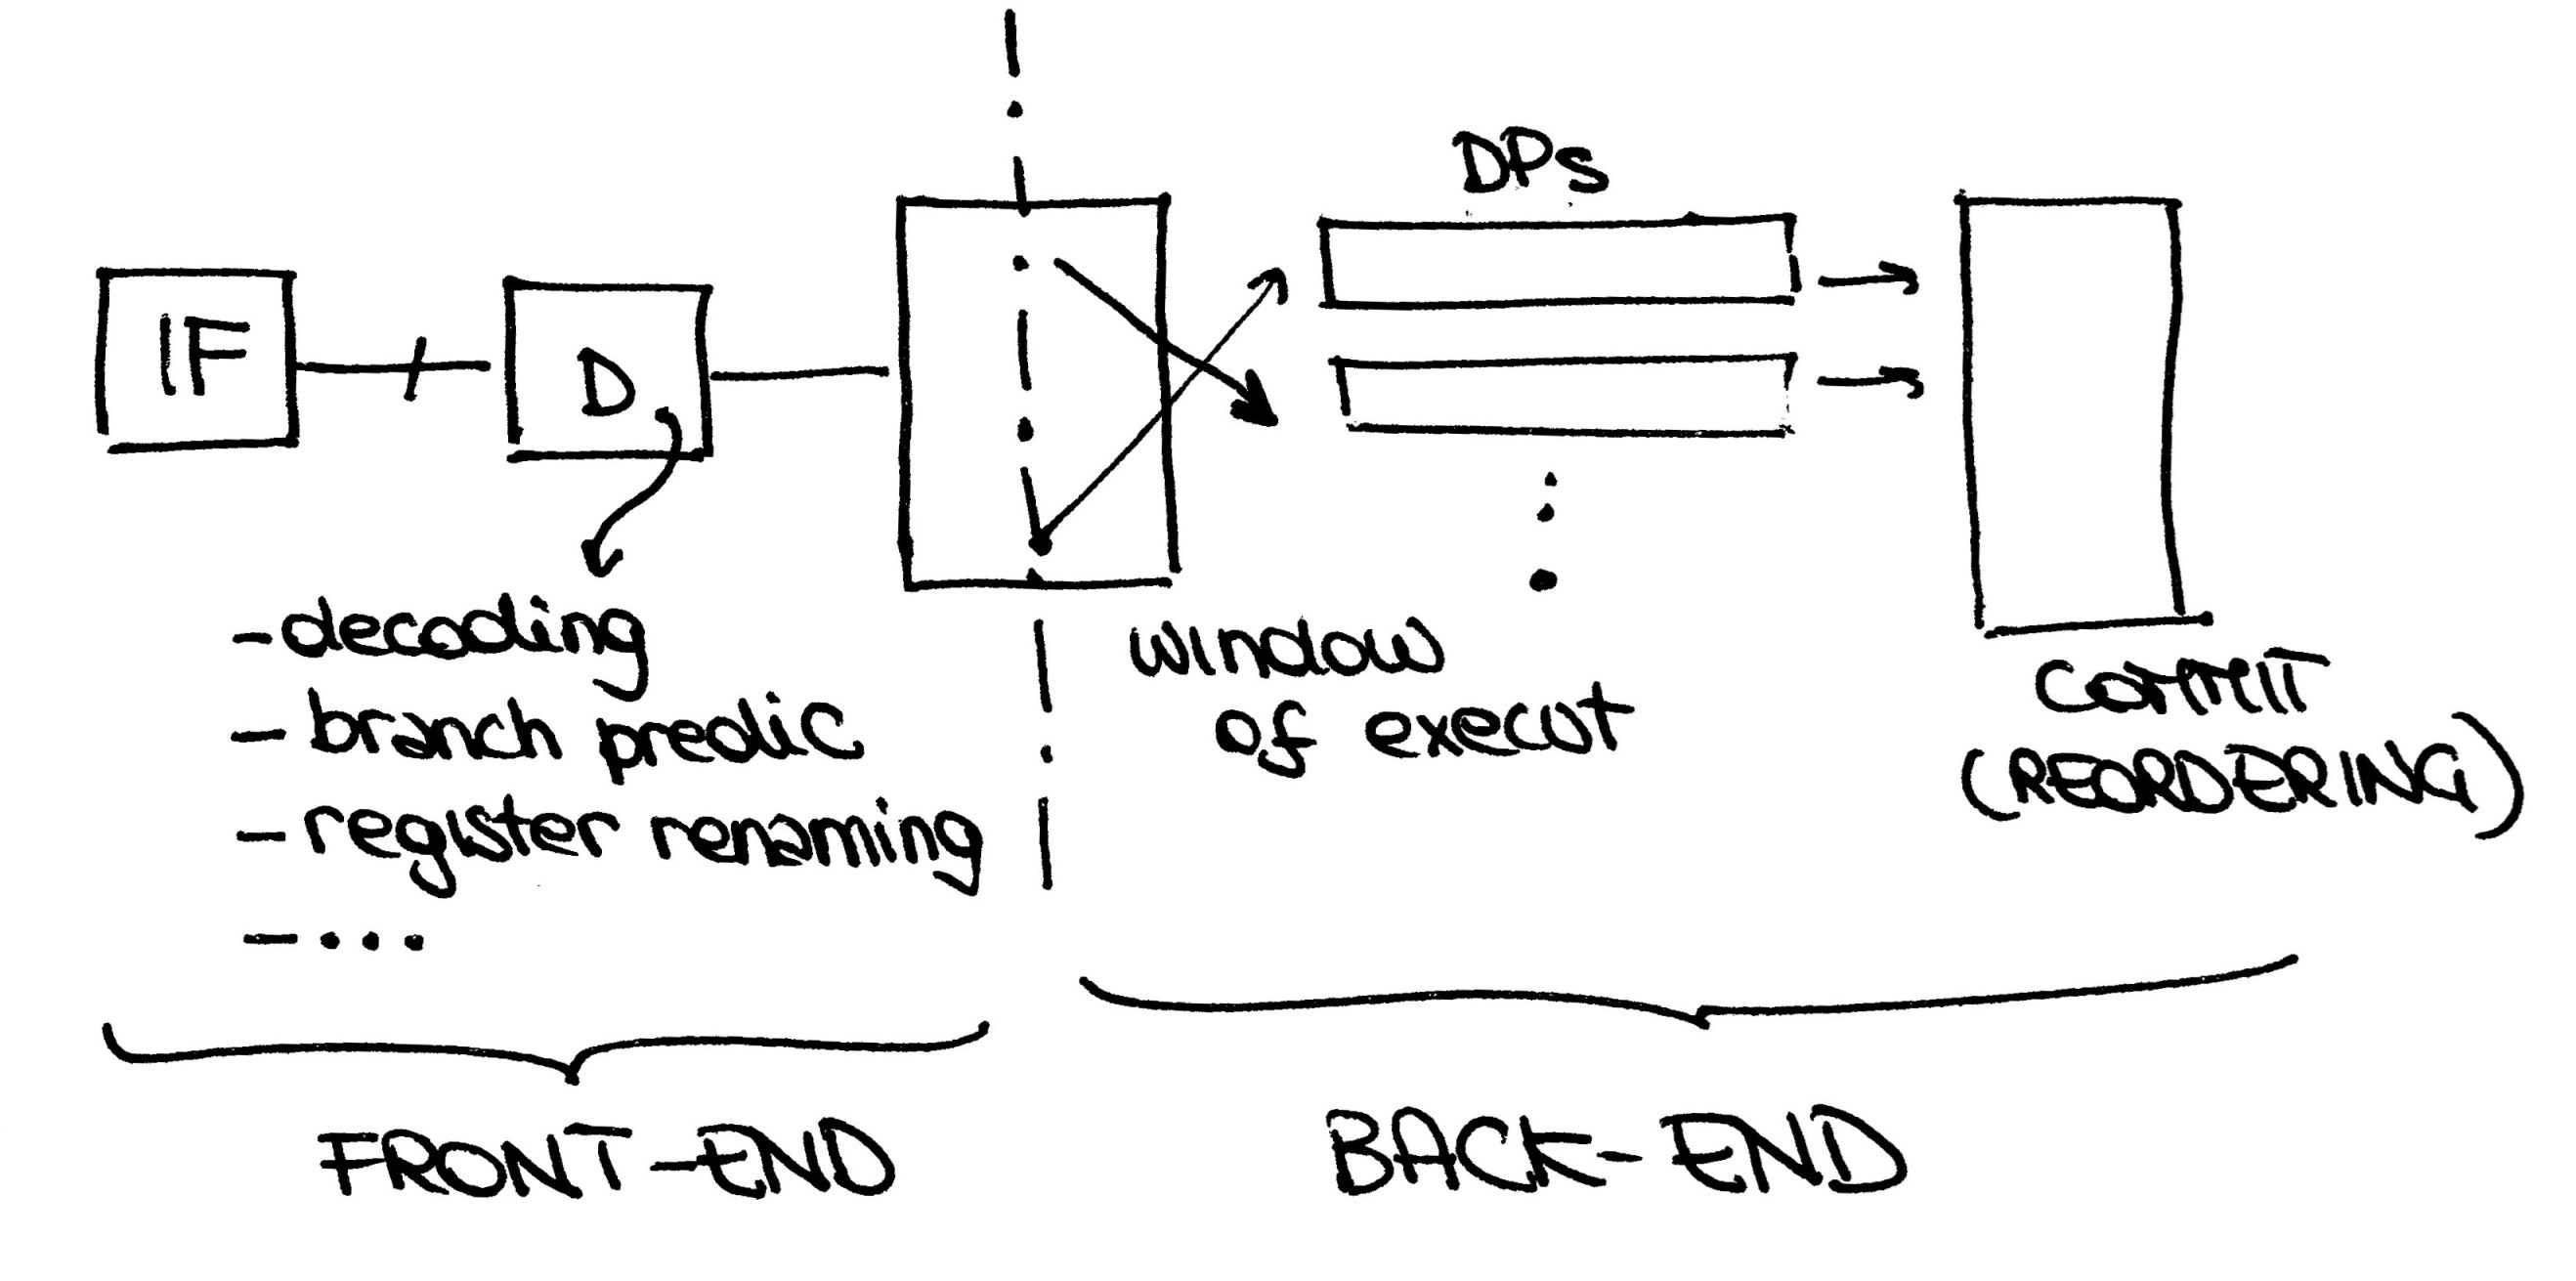
\includegraphics[width=0.7\linewidth]{img/img3/4}
\end{center}

Many different process use the previously seen architecture (like Intel), a
different approach consists of having for each datapath a specific queue,
meaning that each datapath can take instructions only from it's own queue,
which is called \textbf{reservation station}. With this approach we obtain a 
sort of distributed window of execution, the purpose is always the same: extrac
t all the possible parallelism from the instructions, or with a unique buffer 
(window of execution) either with dedicate queues

\begin{center}
  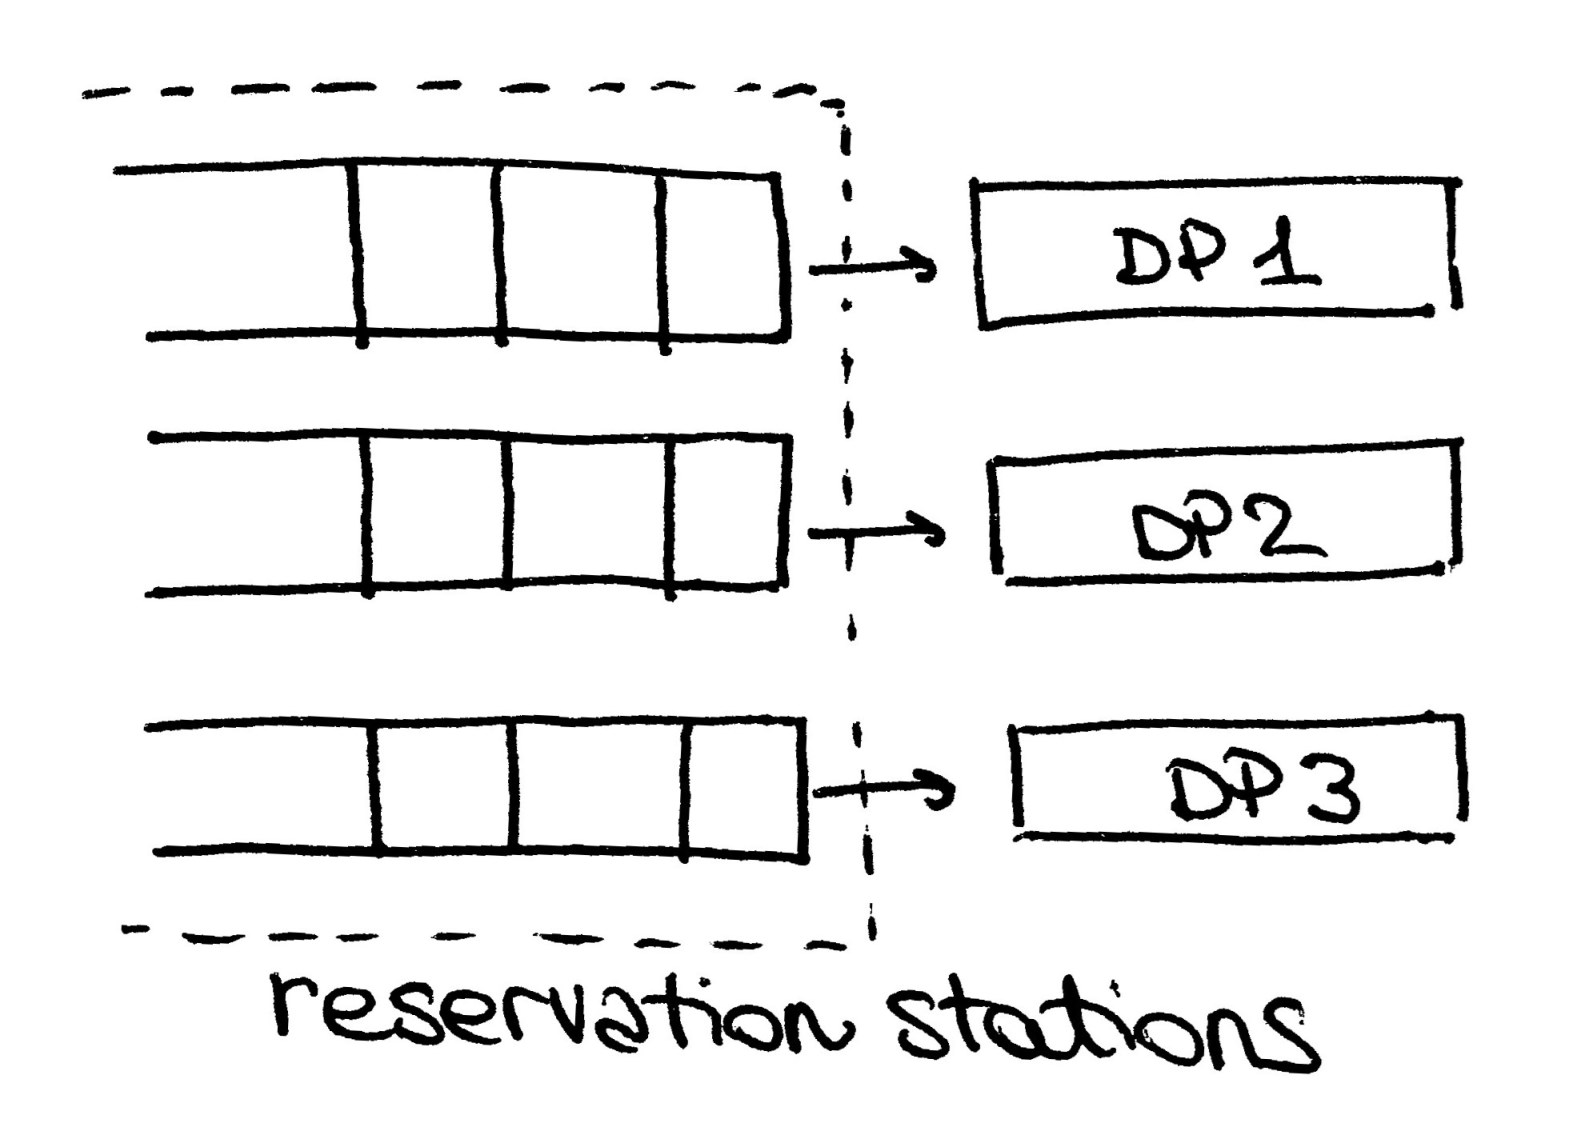
\includegraphics[width=0.5\linewidth]{img/img3/5}
\end{center}

\subsection{Increasing level of parallelism}
To increase the instruction level of parallelism, there are many possibilities:

\begin{itemize}
  \item \textit{Extracts basic blocks and looks at their instructions}. However is difficult achieve a good degree of parallelism since on average 15 \% of instructions are branches or jump, so 1 instruction over 6 is a branch one, leading to have buildings blocks with 5-6 instructions, moreover these 5-6 instructions are usually sequentially so they contain a lot of data dependencies. This means that basic blocks are not sufficient to make the most with a given architecture.

  \item \textit{Branch prediction unit}. The idea is to fill the window of execution or the reservations stations understanding in advance the instructions that will be executed, so we need a prediction and speculation stage, the last one is executing instructions predicted stopping just before the final commit (for the final commit we have to wait).

  \item \textit{Register renaming}: it allows to eliminate data dependencies.

  \item \textit{Change order of execution}: it allows to eliminate data dependencies.
    \subitem \textit{In order processor}: simpler, they don't allow any change with respect to execution order intended by the programmer.
    \subitem \textit{Out of order processor}: they allow dynamic change of instructions order, either in the back-end either in the front end, allowing to exploit better the architecture parallelism.
\end{itemize}

\subsection{Out of order processor}
In order to understand how a out of order processor works, let's take the following example:

\begin{verbatim}
1. ADDF R12, R13, R14
2. ADD  R1, R8, R9
3. MUL R4, R2, R3
4. MUL R5, R6, R7
5. ADD R10, R5, R7
6. ADD R11, R2, R3
\end{verbatim}


Instruction 3 and 4 are potentially in conflict since they employ the same adder while instruction 5 has a data dependency for R5. We assume that all instructions have 1 clock cycle latency except \verb|ADDF| (floating point addition) which has a latency equal to 2.
With term \textit{commit} it is intended the writing of result in the final destination specified by the programmer, with \textit{completion} the instruction has been executed, the result has been stored somewhere, maybe in a temporary register (due to register renaming) but not yet in the final destination.

\subparagraph{Solution 1: in order for both front-end and back-end}
We assume a degree of parallelism for each stage equal to 2.

\begin{center}
  \begin{tabular}{|c|c|c|c|c|c|}
    \hline
    Cycle&    Fetch       &\multicolumn{3}{|c|}{Execution}  &   Completion  \\
    &       &     F.P.  & ADD     & MULT  &               \\ \hline \hline
    1&    $I_1, I_2$&       -&    -&    -&        -\\
    2&    $I_3, I_4$&       $I_1$&  $I_2$&  -&        -\\
    3&    $I_5, I_6$&       $I_1$&  -&    $I_3$&      -\\
    4&      -&          -&    -&    $I_4$&      $I_1,I_2$\\
    5&      -&          -&    $I_5$&    -&      $I_3,I_4$\\
    6&      -&          -&    $I_6$&    -&      $I_5$\\
    7&      -&          -&    -&      -&      $I_6$\\
    \hline
  \end{tabular}
\end{center}

At the end of cycle 2, $I_2$ has finished, the result is already obtained but we cannot perform the completion of $I_2$ since we have to wait for the completion of $I_1$ (strict order both in front end both in back end). In $4^{th}$ cycle we can complete $I_1$ and $I_2$, not $I_3$ since in the completion stage has a degree of parallelism equal to 2.

We cannot start the multiplication of $I_5$ in clock cycle number 4 since it is a in order execution (we have to wait for $I_4$) and due to the data dependencies (R5). Assuming to have a forwarding mechanism we can start $I_5$ just after the end of $I_4$ (we don't have to wait for the completion of $I_4$).

\subparagraph{Solution 2: in order issue and out of order execution}

\begin{center}
  \begin{tabular}{|c|c|c|c|c|c|}
    \hline
    Cycle&    Fetch       &\multicolumn{3}{|c|}{Execution}  &   Completion  \\
    &       &     F.P.  & ADD     & MULT  &               \\ \hline \hline
    1&    $I_1, I_2$&       -&    -&    -&      -\\
    2&    $I_3, I_4$&       $I_1$&  $I_2$&  -&      -\\
    3&    $I_5, I_6$&       $I_1$&  -&    $I_3$&      $I_2$\\
    4&      -&          -&    -&    $I_4$&      $I_1,I_3$\\
    5&      -&          -&    $I_5$&    -&      $I_4$\\
    6&      -&          -&    $I_6$&    -&      $I_5$\\
    7&      -&          -&    -&      -&      $I_6$\\
    \hline
  \end{tabular}
\end{center}


Now we can commit $I_2$ before the completion of $I_1$, however for the final commit we have to wait for $I_1$. Same number of cycles required for solution 1.

\subparagraph{Solution 3: out of order issue and execution}

\begin{center}
\begin{tabular}{|c|c|c|c|c|c|}
  \hline
  Cycle&    Fetch       &\multicolumn{3}{|c|}{Execution}  &   Completion  \\
  &       &     F.P.  & ADD     & MULT  &               \\ \hline \hline
  1&    $I_1, I_2$&    -    & -   & - &         -     \\
  2&    $I_3,I_4$&        $I_1$&  $I_2$&  -&            -     \\
  3&    $I_5,I_6$&        $I_1$&  -&    $I_3$&          $I_2$   \\
  4&      -&          -&    $I_6$&  $I_4$&          $I_1, I_3$  \\
  5&      -&          -&    $I_5$&  -&            $I_6, I_4$  \\
  6&      -&          -&    -&    -&            $I_5$   \\
  \hline
\end{tabular}
\end{center}

With this solution we are saving one cycle since we can swap the order in the completion and in the execution stage, issuing $I_6$ before $I_5$.


\section{VLIW}

Using VLIW approach, instructions are executed in parallel but the parallelism is exploited during compilation (static view). Summarizing what we have already seen:\\

In super-scalar approach:
\begin{itemize}
  \item Everything is done dynamically by the processor, for the compiler everything is transparent since every kind of problem is detected and solved by hardware.
  \item Binary compatibility: we can still execute the binary code compiled for a previous version of the processor since compiler doesn't need a complete knowledge on processor.
  \item To exploit instruction parallelism in hardware a lot of complex units are required.
\end{itemize}

In VLIW approach:
\begin{itemize}
  \item Compiler detects ILP (instruction level parallelism), since it can access to much more memory where store the window of execution, a greater level of parallelism can be exploited.
\end{itemize}

\subsection{VLIW Scheme}
\begin{center}
  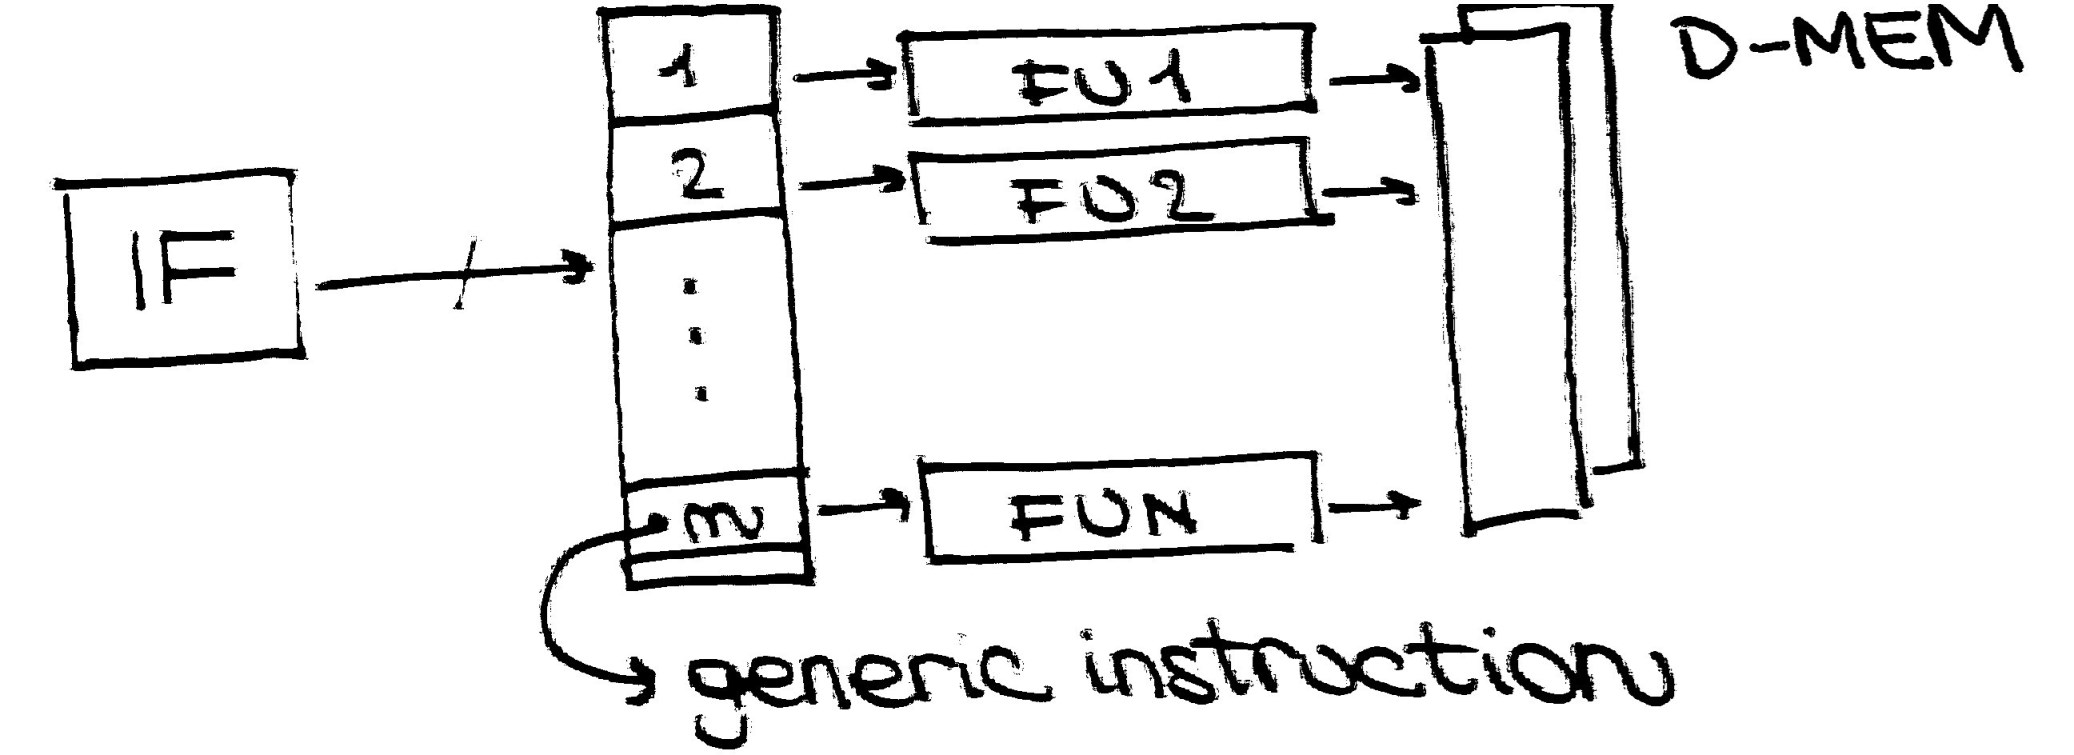
\includegraphics[width=0.7\linewidth]{img/img3/6}
\end{center}


It is just needed to take $n$ instructions from the instruction memory and dispatch them to the functional units, so no branch detection or data dependencies are required, everything has already been checked. Then it is possible to specialize the function units, so maybe FU1 is a floating point unit, FU2 is a divisor, etc. It is required a lot of bandwidth versus instruction memory, RF and data memory but the hardware is much simpler. However it is quite common that the compiler is not able to feed at each clock cycle every functional units (due to data dependencies, the fact that only one divisor is available, and so on), this implies that a lot of words composing the fetched  instruction are empty/wasted.

\subsection{Compressing instruction memory}
One possible solution is to decrease the amount of instruction memory required (since may words will be empty), compressing the information.

\begin{center}
  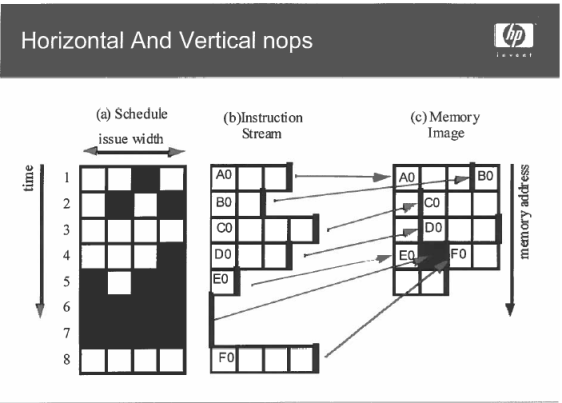
\includegraphics[width=0.8\linewidth]{img/img3/compr1}
\end{center}

A $U$ means that the FU (Functional Unit) is used, $X$ that is not. Compression is performed in two steps: in horizontal compression we align to the right all $X$ (which are nops) and for each row we add a template (i.e. a binary pattern) to say that in row 1, the first 3 U are referred to FU1, FU2 and FU4 for instance, then in vertical compression (second stage) empty rows are canceled.\\

To uncompress: the processor will reads 4 fields at the same time, if all of them are referring to different FU they can be all dispatched, instead if some of them referred to the same FU, the processor has to postpone them.

\begin{center}
  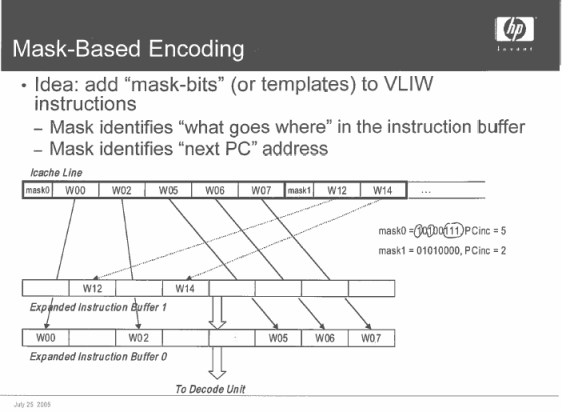
\includegraphics[width=0.8\linewidth]{img/img3/compr2}
\end{center}

After fetching the instructions, processor accesses to the mask:
mask0= 10100111

Having 8 functional units:

\begin{verbatim}
mask0(0)=1 ->  W0 in  FU0
mask0(1)=0 ->  NOP in FU1
mask0(2)=1 ->  W2 in FU2
...
\end{verbatim}

Adding mask bits (as many as the number of functional units) it is possible to obtain a significantly memory saving.

\section{TTA architecture}

Standing for Transport Triggered Architecture, the idea is based on the fact that every kind of processing can be translated into moves (meaning to take data from some source and move to a certain destination). Taking as example:

\begin{verbatim}
ADD   R1  R2  R3
\end{verbatim}

In TTA approach, before exploit parallelism we translate the starting instruction into a sequence of move.

\begin{center}
  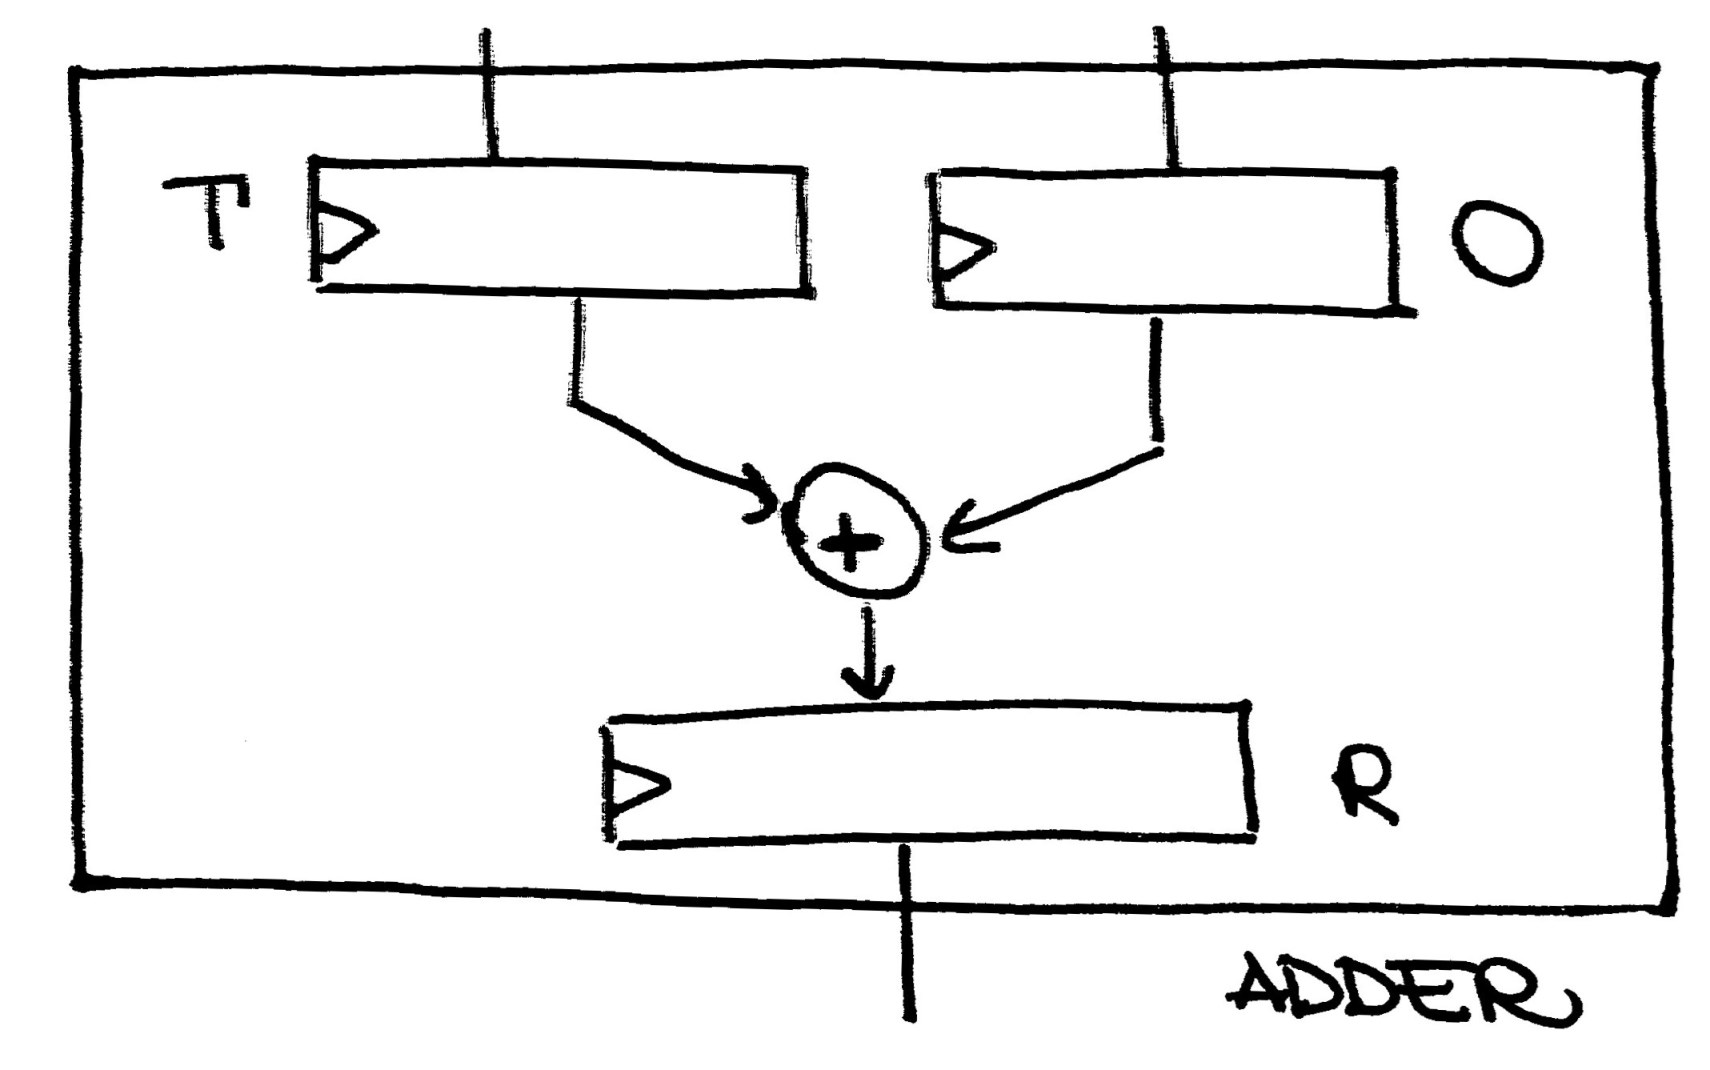
\includegraphics[width=0.5\linewidth]{img/img3/7}
\end{center}

Suppose that this new adder has two input registers and provide the output on a given register, the original operation can be translated as:
\begin{verbatim}
MOVE  o R2
MOVE  T R3
MOVE  R1  R
\end{verbatim}

Where \verb|T| is a special register so that when it is loaded it can trigger the operation. If all functional units are organized like that (including RF and data memory) then we can translate all instructions into move operations.\\

The instruction set just consists of one instruction (i.e. move), the compiler is responsible for translating into moves and organized them in parallel the instruction sequence. It is possible to exploit pipelining if the operation is more complicated than a simple addition.

\begin{center}
  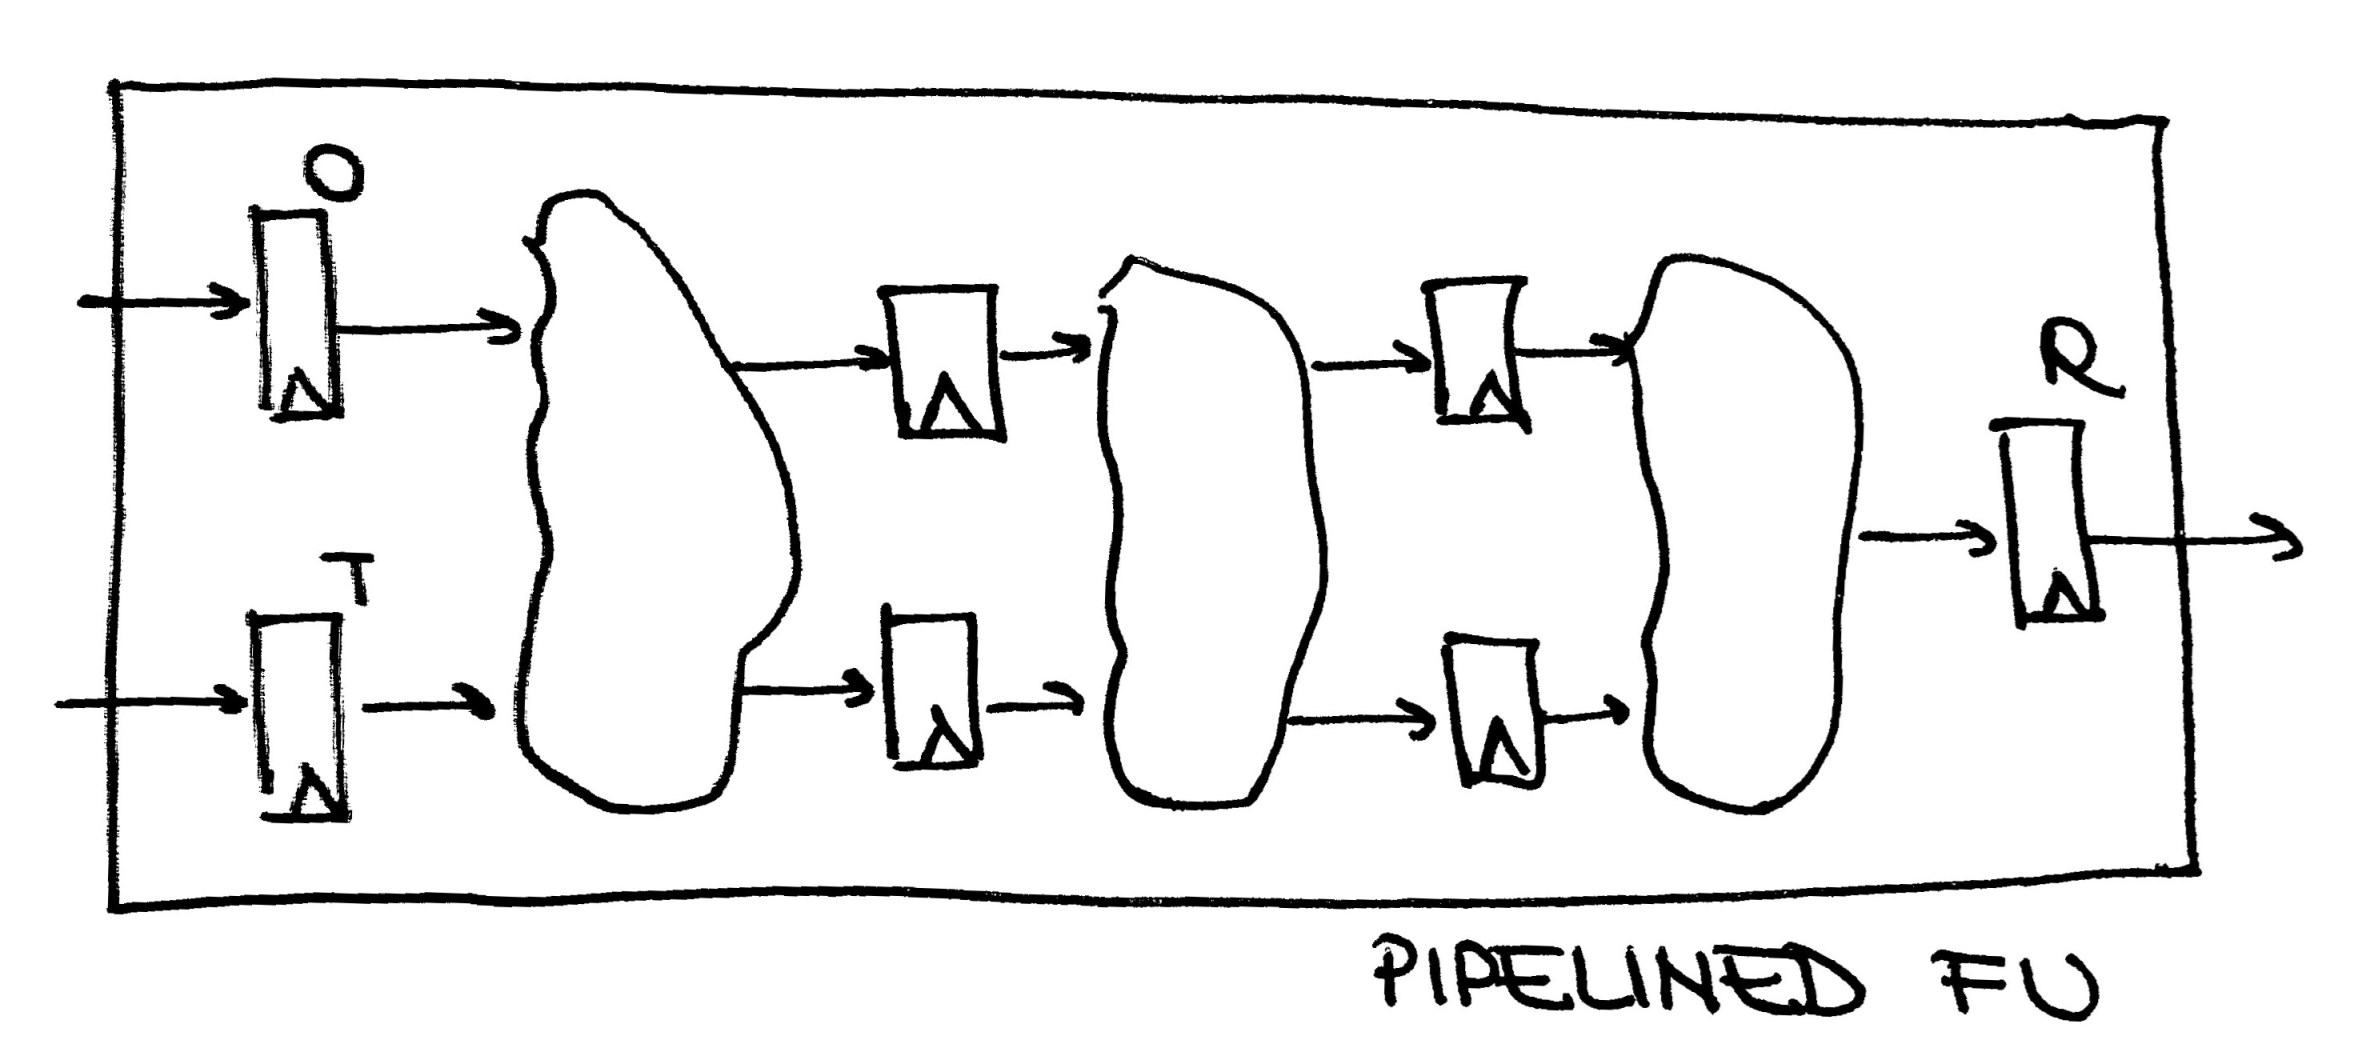
\includegraphics[width=0.7\linewidth]{img/img3/8}
\end{center}

In this way the compiler knows the internal latency of each functional unit. It is also required a proper number of buses to perform all move operations in parallel.

\begin{center}
  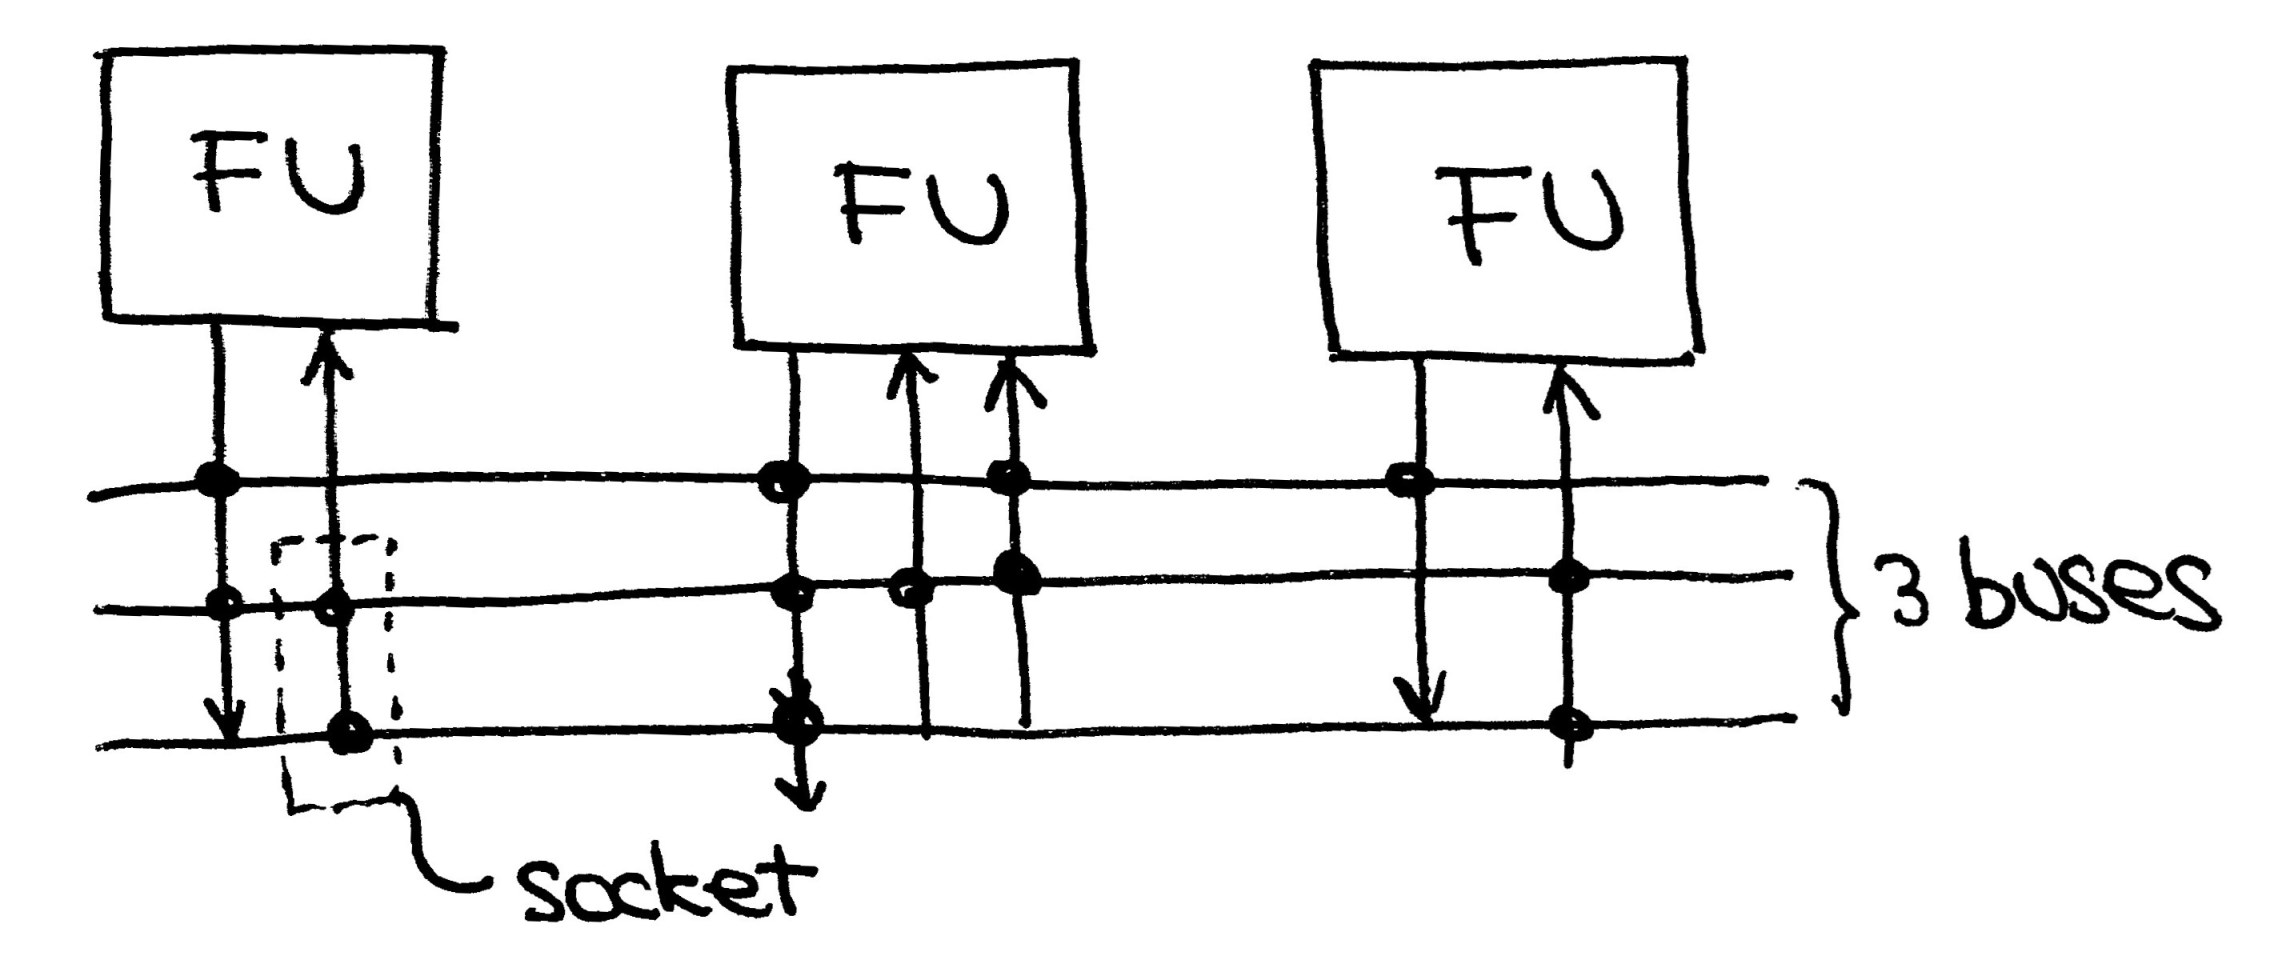
\includegraphics[width=0.7\linewidth]{img/img3/9}
\end{center}

If we have 3 buses in parallel it means that we can perform up to 3 moves in parallel. Socket is the pattern for each input/output of a functional unit that determine to which buses this I/O is connected.

\subsection{Software bypassing}

It is like a hardware forwarding, taking as an example:

\begin{verbatim}
ADD R3  R1  R2
ADD R5  R1  R3
\end{verbatim}

And translating them into moves operation:

\begin{verbatim}
MOVE  O   R1
MOVE  T R2
MOVE  R3  R
MOVE  O R1
MOVE  T R3
MOVE  R5  R
\end{verbatim}

Compiler should be able to recognize two things:
\begin{enumerate}
  \item This two instructions have a common operand, so to achieve a faster execution we can remove the move command for $R1$ (instruction 4 can be canceled).
  \item There is a data dependency since we need the result of first addition as input of the second, so we can directly move it to T register.
\end{enumerate}

This leads to:
\begin{verbatim}
MOVE  O   R1
MOVE  T R2
MOVE  T R
MOVE  R5  R
\end{verbatim}

As optional we can put \verb|MOVE R3 R| between 3 and 4 depending on variable life time. These kind of optimizations are easily performed by compiler.

\begin{verbatim}
\# larger example



















\end{verbatim}

It is required to tune the processor to perform a number of move in parallel: this amount depends on socket patterns and number of buses (they are responsible for optimization).

Connecting all i/o ports of a functional units to all buses may lead to a waste of power: the optimal architecture is the one with the minimum number of dots and no performance penalty.

This kind of architecture is common in ASIP.

\section{ASIP}
Standing for Application Specific Instruction set Processor, the kind of task is always the same, like a processor connected to the ABS in a car, or a TV decoder (more complex but it is always the same). For this processor family it makes sense optimize the architecture, maintaining the capability to program it.
To implement asip a common solution is using TTA architecture since it can be very well optimized.
Depending on the application, we allocate a certain number of functional units, buses and all possible connections (quite expensive approach):
\begin{verbatim}
\# starting point for the optimization flow


















\end{verbatim}
Then we can simulate it and measure the percentage use of each kind of resources, based on this analysis the architecture can be simplified by removing the least used resources.

\# img

Starting from a high implementation cost and a low delay we can remove units up to the point when performances start to decrease significantly.

Summarizing:

\begin{enumerate}
  \item The initial processor is very similar to a mips, (risk based with 5 pipeline stage) with a certain ISA. To enhance it, we can provide the ISA with a more powerful instruction for a certain application (like fft): this leads to a dedicated hardware (i.e. specialized function unit) that perform the fft and can be used by a special instruction.

  \item Starting from a given template processor, we can tuned it on our requirements (numbers of stages, at which stage allocate the elements we want, etc), just limiting to a pipelined organization (no VLWI architecture).
\end{enumerate}

\section{Super Scalar Processors}

For a  in order processor all operations in each stage have to been performed
in the exact order intended by the programmer. The processor we used as an
example to understand basic steps was made by DEC and called ALPHA21164. Its
architecture is based on 4-way (4 datapath in parallel), load/store (similar to
MIPS for memory access). Block level diagram is the following:

\begin{center}
  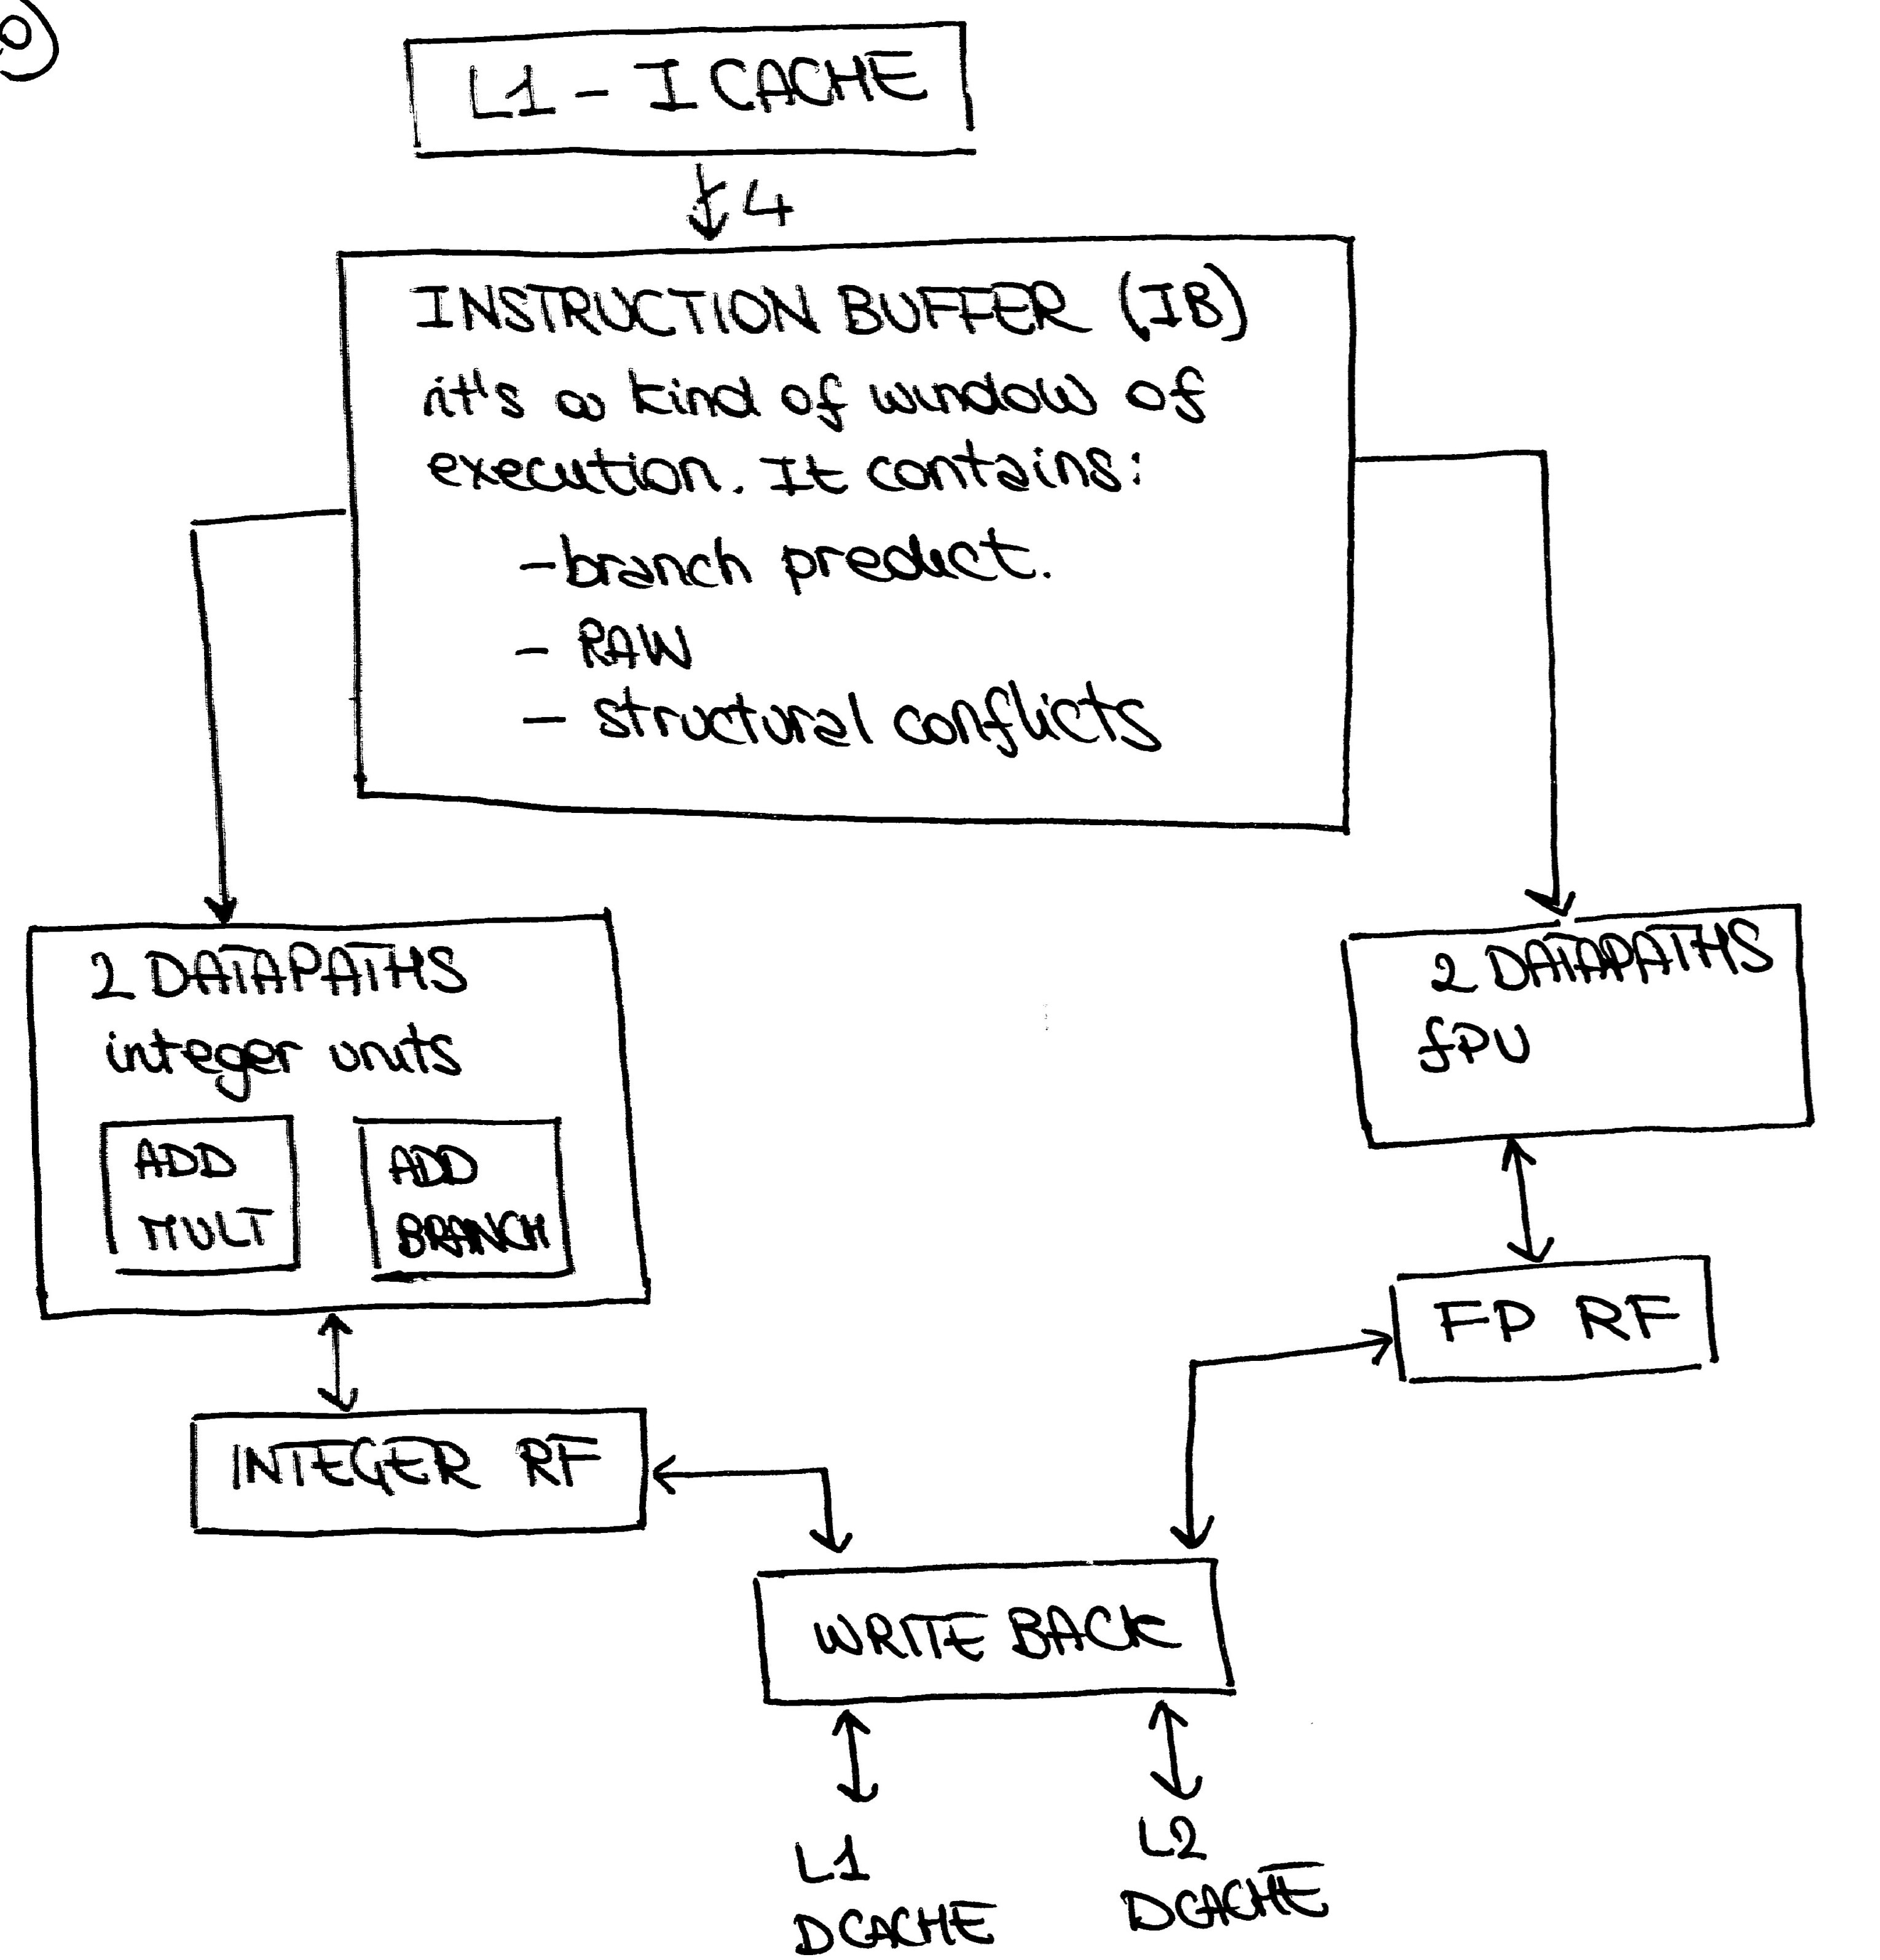
\includegraphics[width=0.7\linewidth]{img/img3/10}
\end{center}

Looking at this organization it can be noticed that for the front end there are
4 pipeline stages while execution units have not the same amount of pipeline
stages, meaning that for an integer operation (FU1 and FU2) there are three
stages while for floating point unit (FU3, F4)  5 stages are placed. By
focusing on these stages we have that front end is made up of $s_0,s_1,s_2, s_3$
while execution units have $s_4,s_5,s_6$ for integer operations and
$s_4,...,s_8$ for floating point ones.\\

In particular regarding front end stages:

\begin{itemize}
  \item $s_0$: access to I-cache to take 4 instructions at the same time.
  \item $s_1$: validation of read instruction and branch prediction (we have
  to handle it as soon as we have the instructions to anticipate as much as
  possible the branch direction and the target address).
  \item $s_2$: structural hazards, for instance if all 4 operations regard
  integer operation 2 of them have to been stopped.
  \item $s_3$: dynamic conflict, in particular since it is a in order
  processor just RAW conflicts may occur, so we verify that all input
  operands for a certain operation are actually available.
\end{itemize}

\subparagraph{RAW conflict example}
Let's consider the following example:
\begin{verbatim}
I1: R1 <- R2+R3
I2: R4 <- R1-R5
I3: R7 <- R8-R9
I4: F0 <- F2+F4
\end{verbatim}

Between I1 and I2 there is a RAW conflict and three instructions regard integer
data, we can proceed to execute the operations in the following way:

\begin{center}
  \begin{tabular}{|c|c|c|c|c|}
  \hline
  Cycle&    Stage 0&    Stage 1&      Stage 2&    Stage 3\\
  \hline
  1&    I1, I2, I3,I4&    - &         - &         -\\
  2&    I5,I6,I7,I8&    I1, I2, I3,I4&    -&          -\\
  3&    ...&        I5,I6,I7,I8&    I1, I2, I3,I4&    -\\
  4&    ...&        ...&        I5,I6,I7,I8&    I1, I2\\
  \hline
  \end{tabular}
\end{center}

In clock cycle number 4, since only two integer units are available, we can
only process I1 and I2, so I3 has to be stopped and I4 cannot be started since
it is a in order processor (before we have to start I3). In the following step,
instruction I2 is stopped due to RAW conflict, so although we have 4 parallel
datapath we have to stall some operations.\\

Typically Stage 2 and Stage 3 are the so called scoreboarding.

\subsection{Load-store instruction stages}
The pipeline stages involved in load or store instructions are stage 4 in which
address calculation is performed and stage 5 in which access to data-cache
actually occurs. Two possibilities:

\begin{itemize}
  \item \textbf{Hit}: for a reading instruction data is available at the end
  of Stage 5, for writing the operation is completed in Stage 6.
  \item \textbf{Miss}: in this case we have to go in L2 cache, so in addition
  to Stage 5 and Stage 6 we require 6 more stages to support the latency
  versus L2 cache (up to Stage 12).
\end{itemize}

\subsection{Branch}
In stage 4 the condition for branch is evaluated and in stage 5 branch can be
resolved, however some other instructions have already been fetched. At this
point we have to check if the prediction was correct, if it was
everything is fine, if it was not we have to discharge everything from stage 0
to stage s4; since 4-instructions parallelism is supported a big penalty
rises with wrong prediction.

\subsection {Scoreboarding}
\begin{center}
  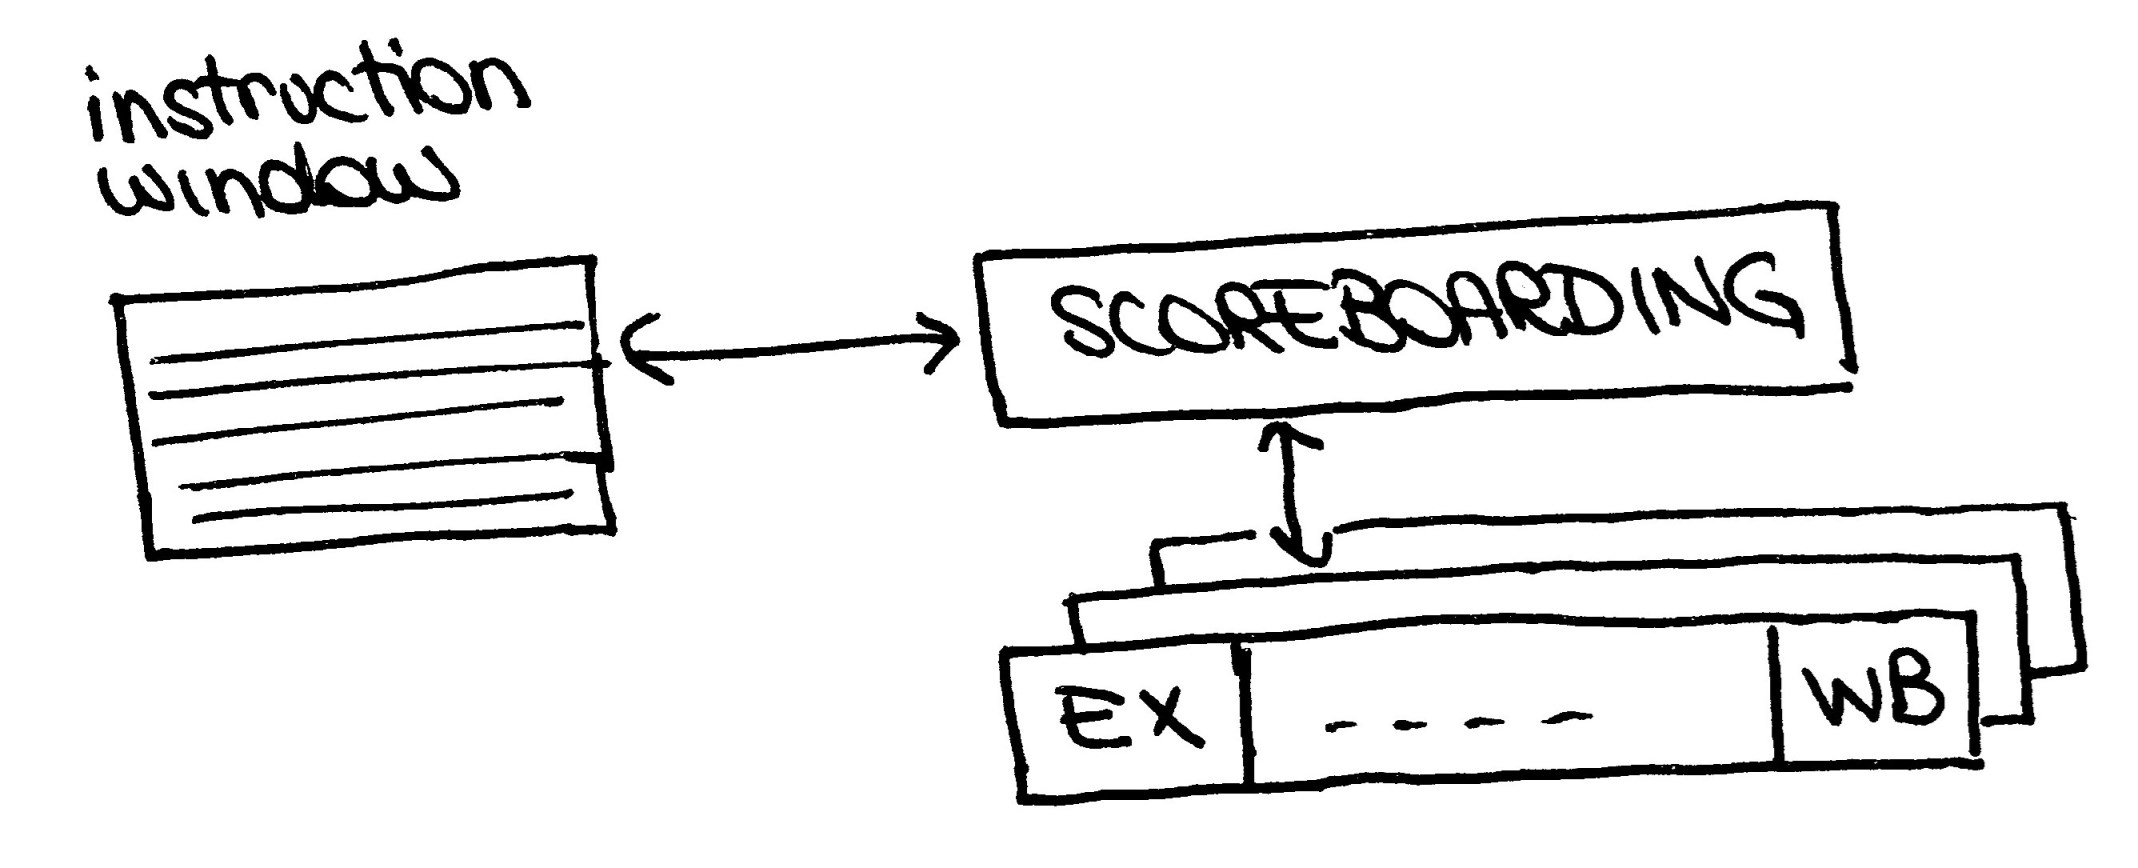
\includegraphics[width=0.7\linewidth]{img/img3/11}
\end{center}

To study the scoreboarding unit we will not analyze DEC alpha one but a more
complete which is able to handle also other kind of conflicts (not only RAW).
It is made up of several stages:
\begin{enumerate}
\item \textbf{Issue step}
  \subitem Check for structural hazards.
  \subitem Check for WAW.

If these two checks are passed instruction is issued, otherwise it remains in
this stage.

\item \textbf{Read or dispatch step}
  \subitem Read operands.
  \subitem Check for RAW.

\item \textbf{Execution step}
\item \textbf{Write step}
  \subitem WAR conflict detection.
\end{enumerate}

If any of these checks is not passed, the instruction has to be kept in that
stage until it passes.

\subsubsection{Scoreboard data structures}

Some data structures are allocated in the scoreboarding unit:

\begin{itemize}
\item \textbf{Instruction status table}
\begin{center}
  \begin{tabular}{|l|c|c|c|c|}
    \hline
    Instruction&  Issue&    Read&  Execution&   Write\\
    \hline
    Instr. 1  & & & &  \\
    Instr. 2  & & & &  \\
    Instr. 3  & & & &  \\
    Instr. 4  & & & &  \\
    \hline
  \end{tabular}
\end{center}

For each instruction we have to sign its status for the different scoreboard
steps.

\item \textbf{Functional unit status table}
Each row corresponds to a specific functional unit:

\begin{center}
  \begin{tabular}{|l|c|c|c|c|c|c|c|c|c|}
    \hline
    FU &Busy& Op &  Dest.reg ($F_i$)& Source reg 1
    ($F_j$)&
    Source reg 2 ($F_k$)& $Q_j$& $Q_k$& $R_j$&  $R_k$\\
    \hline
    FU1 & & & & & & & & & \\
    FU2 & & & & & & & & & \\
    FU3 & & & & & & & & & \\
    FU3 & & & & & & & & & \\
    \hline
\end{tabular}
\end{center}

$Q_j$ and $Q_k$ contain the name of the functional units that will generate
the value to be written in $F_j$ and $F_k$ (needed for forwarding), $R_j$ and
$R_k$ are valid data flag.

\item \textbf{Register result status table}

F0    F1    F2    ..
| |   |

F0, F1, F2... are registers and for each of them we report which functional
unit will provide the value to be written in that register.
\end{itemize}

So summarizing all these operations:

\begin{center}
  \begin{tabular}{|l|p{7 cm}|p{7 cm}|}
    \hline
    Step &    Condition check &   Actions (if all checks are passed)\\
    \hline
    Issue &   \begin{itemize}
          \item FU free?
          \item WAW
          \end{itemize} &     \begin{itemize}
                      \item Set FU busy.
                      \item Record $F_i, F_j, F_k, Q_j, Q_k, R_j, R_k$.
                      \item Store FU name in RF.
                      \end{itemize} \\

    Read&   RAW conflict exists if either $R_j$ or $R_k$ is equal to 0.&
          Send $F_j, F_k$ to the selected FU. \\

    Execution&- & - \\
    Write&    WAR conflict($F_i$ for one instruction, for
    the other instructions already issued
    $F_j$ and $F_k$).& - \\
    \hline
  \end{tabular}
\end{center}

\subparagraph{Example}
The following set of instructions has to be performed:

\begin{verbatim}
I1:   R4 <- R0 X R2
I2:   R6 <- R4 X R8
I3:   R8 <- R2+R12
I4:   R4 <- R14 + R16
\end{verbatim}

where I1 and I2 are multiplications. Some conflicts exist:
\begin{enumerate}
  \item I2-I1: RAW.
  \item I2-I3: WAR.
  \item I1-I4: WAW.
  \item All structural hazards.
\end{enumerate}

We assume that addition takes 1 single cycle while multiplication required 5 cycles.

\begin{verbatim}
\# img/tabelle per cycle



















\end{verbatim}

\textit{Cycle 1}: in $Q_j$ and $Q_k$ fields we put "?" since we don't know who actually wrote the source registers but we assume that they are already available since $R_j=R_k=1$.\\

\textit{Cycle 2} looking at R6 in the register result status, since this field is equal to 0 it means that there are no other instructions in the scoreboard who want to write their own result in R6; this implies that no WAW conflict occurs for I2.\\

The operation of checking WAW is not only a read and compare but it is a search in tables, meaning that given the destination register (which is easy to find) we have to look at all source registers for each FU to find a match. A sequential read operation may take time so the table should be organized as an associative memory (at least one part of functional unit states table) in order to be able to tell us if a certain word is present or not (although it is a much more expensive).\\

At cycle 9 we have to flush rows regarding instruction 1 since it is finished.


%%%%%%%%%%%%%%%%%%%%%%%%%%%%%%%%%%%%%%%%%%%%%%%%%%%%%%%%%%%%%%%%%%%%%%%%%%%%%%%%
%%%%%%%%%%%%%%%%%%%%%%%%%%%%%%%%%%%%%%%%%%%%%%%%%%%%%%%%%%%%%%%%%%%%%%%%%%%%%%%%
%%%%%%%%%%%%%%%%%%%%%%%%%%%%%%%%%%%%%%%%%%%%%%%%%%%%%%%%%%%%%%%%%%%%%%%%%%%%%%%%

\section{Superscalar out of order processors}
To increase instruction level parallelism out of order processor are exploited;
for them a number of additional features have to be allocated, in particular the
most important one is register renaming.

%%%%%%%%%%%%%%%%%%%%%%%%%%%%%%%%%%%%%%%%%%%%%%%%%%%%%%%%%%%%%%%%%%%%%%%%%%%%%%%%
%%%%%%%%%%%%%%%%%%%%%%%%%%%%%%%%%%%%%%%%%%%%%%%%%%%%%%%%%%%%%%%%%%%%%%%%%%%%%%%%
%%%%%%%%%%%%%%%%%%%%%%%%%%%%%%%%%%%%%%%%%%%%%%%%%%%%%%%%%%%%%%%%%%%%%%%%%%%%%%%%

\subsection{Register renaming}
To understand how register renaming works, let's look at the following list of instructions:
\begin{verbatim}
i1  R1=R2/R3
i2  R4=R1+R5    RAW with I1
i3  R5=R6+R7    WAR with I2
i4  R1=R8+R9    WAW with I1
\end{verbatim}

By register renaming we can eliminate the last two data dependencies (the first one cannot be eliminated). In order to apply this technique we have to distinguish between registers seen by the programmer \textbf{logical registers} (R1, R2,..., the ones in RF) and \textbf{physical registers} which are not seen by the programmer. The fist operation is therefore to translate logical registers into physical register (assuming that physical registers are the ones multiple of 10):

\begin{verbatim}
i1  R10 = R20/R30
i2  R40 = R10+R50   RAW with I1
i3  R50=R60+R70   WAR with I2
i4  R10=R80+R90   WAW with I1
\end{verbatim}

The first conflict cannot be eliminated, but for the second two it's sufficient change R50 in I3 into R51 and rename all source operands equal to R50 starting from I3 into R51.

\begin{verbatim}
i1  R10 = R20/R30
i2  R40 = R10+R50   RAW with I1
i3  R51=R60+R70
i4  R11=R80+R90
\end{verbatim}

To perform register renaming at run time:
There is a list of available physical registers, the access to the first available location is made using pointer \verb|ptr|, in this way we are able to perform $R_i \rightarrow R_a$.
Then a rename table is addressed by logical register returning the corresponding physical register. So regarding destination register we first have to find an available physical register, increment the pointer (so it will point at the following location of free list), perform two read operations on the renaming table for 2 source registers and finally a writing operation on the same table to save where the destination register is actually stored.

\begin{center}
  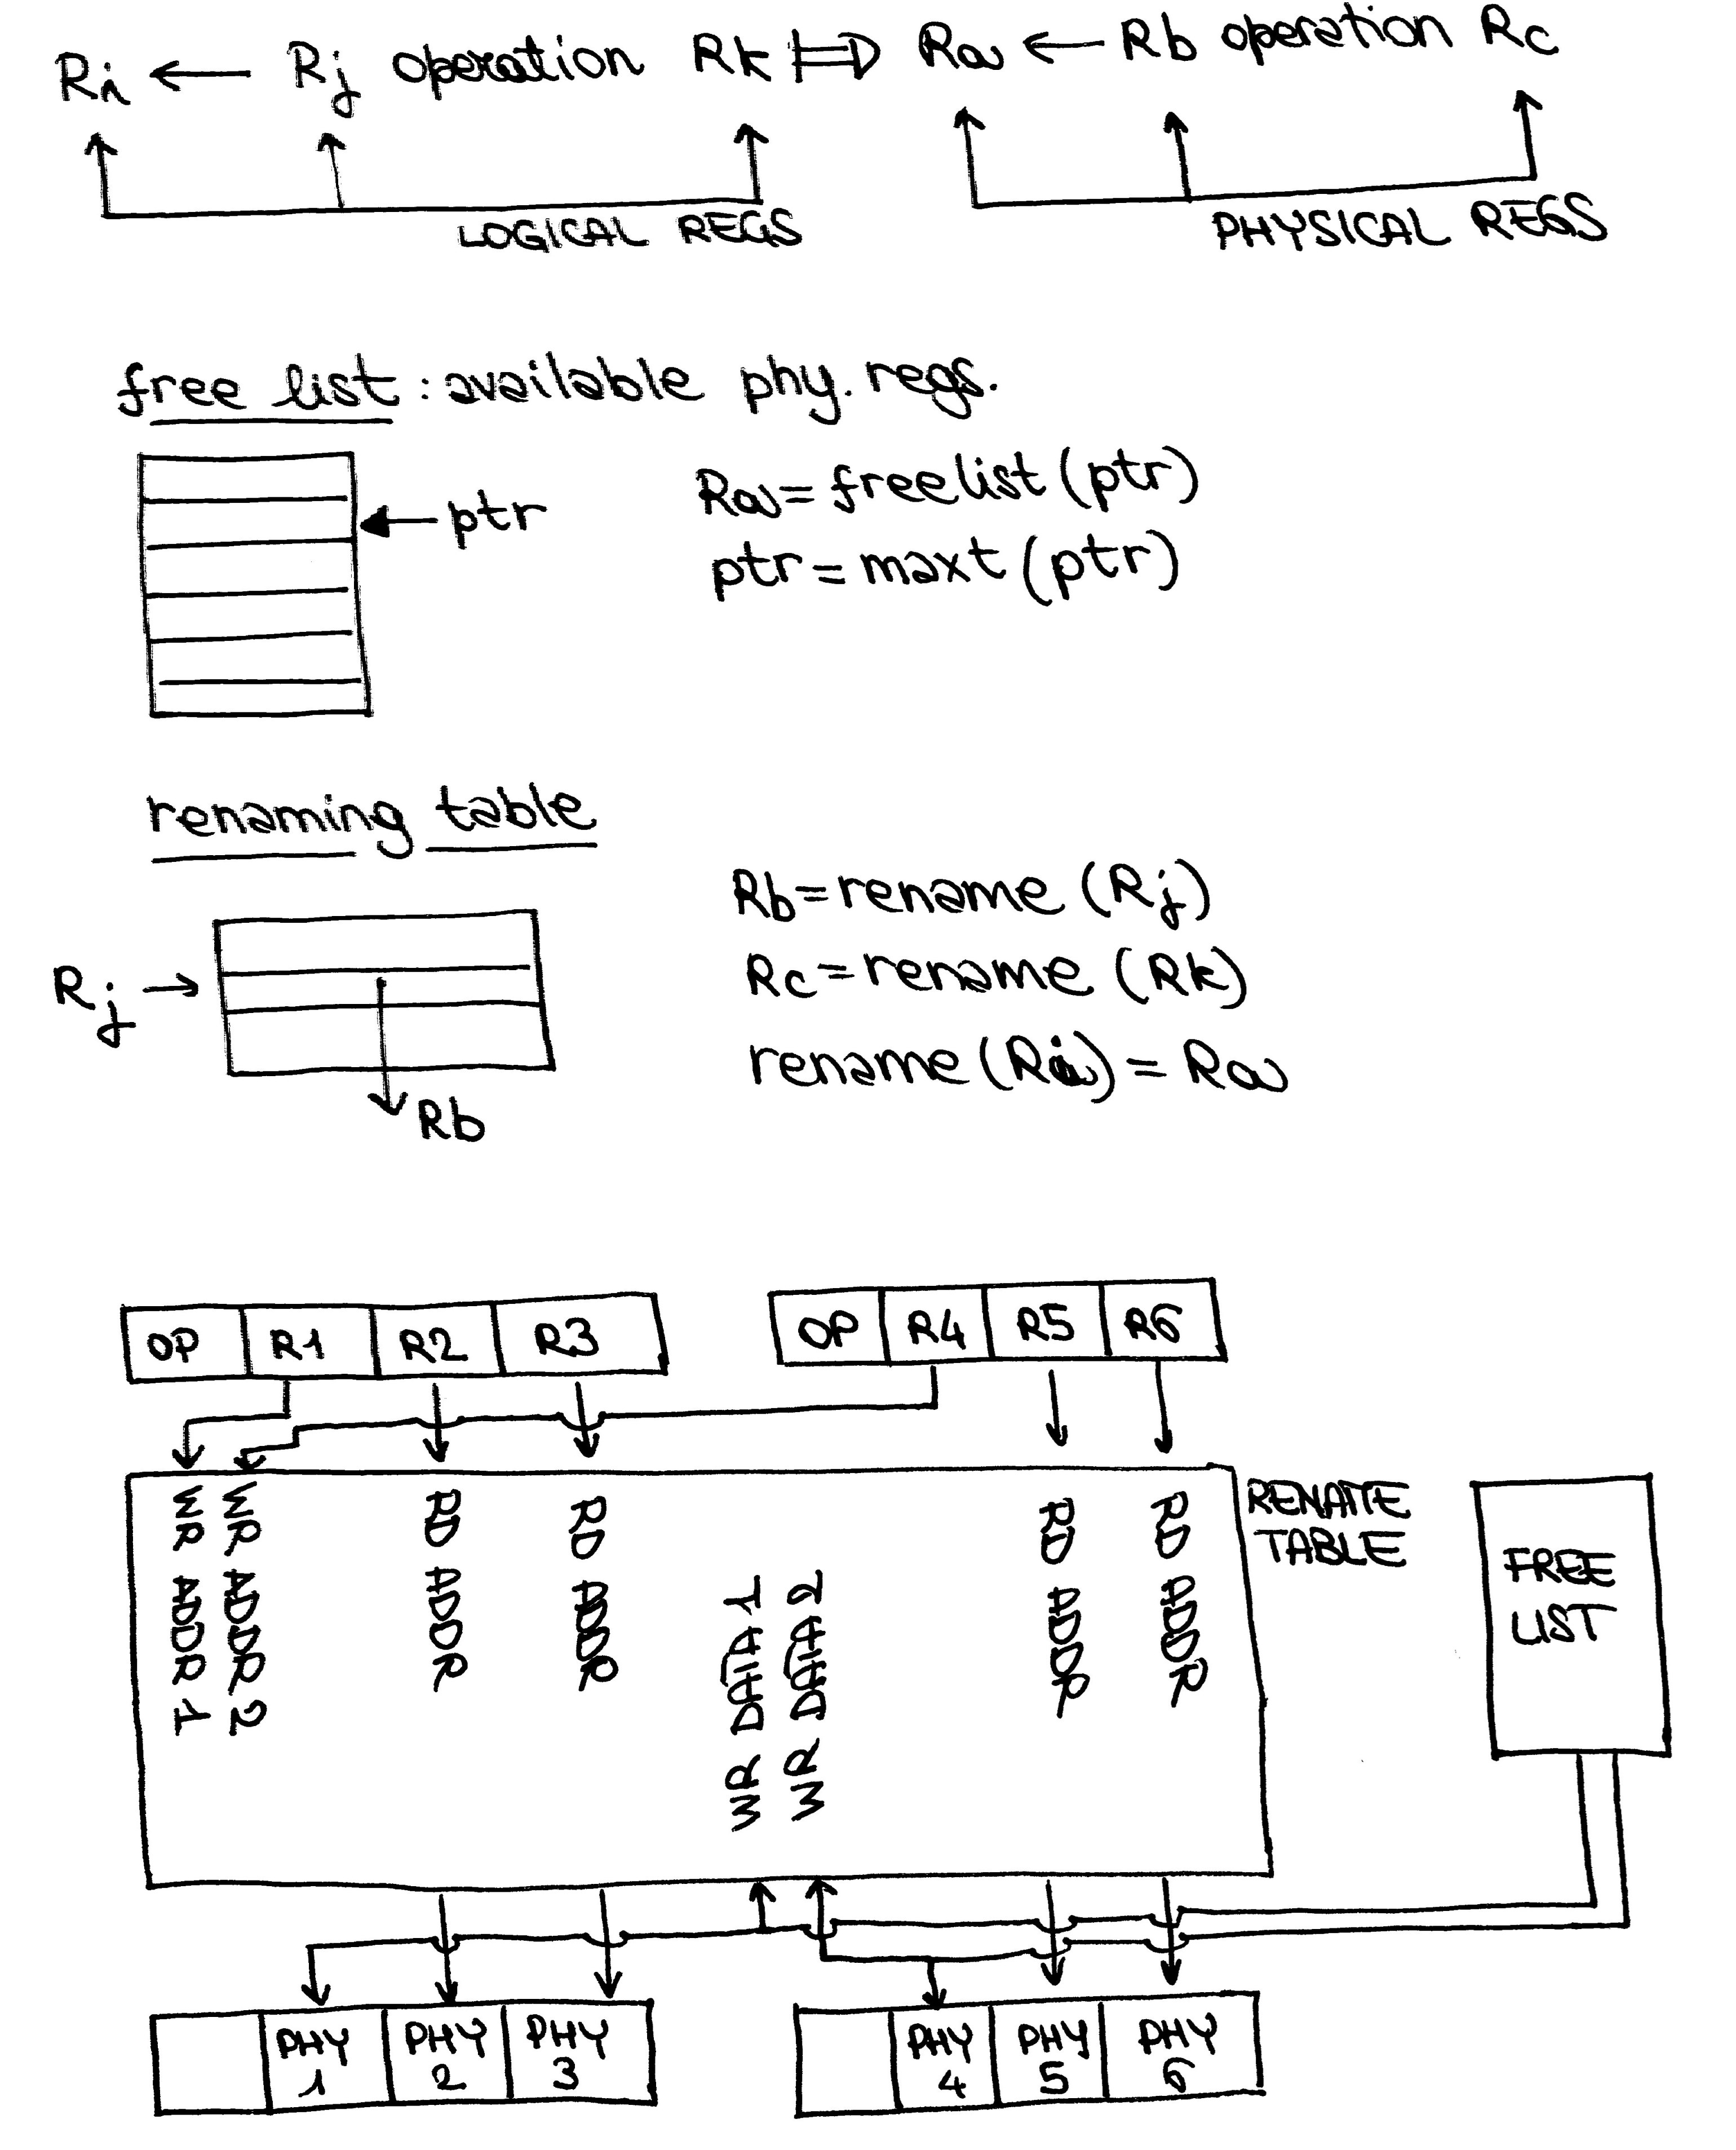
\includegraphics[width=1.0\linewidth]{img/img3/26}
\end{center}



However we may have RAW conflicts which cannot be eliminated; the point is that the renaming unit doesn't have to mask this conflict. It means that in the previous example we have two instructions where the second one having \verb|op r4 r1 r6| so a RAW conflict is present. When we access the renaming table for \verb|r1| (source register in second operation) the content of that location has not still been updated by the writing of the first operation. So for the output of the second operation we have to take either the renaming table either the free list depending on the fact that a RAW occurs.

\begin{center}
  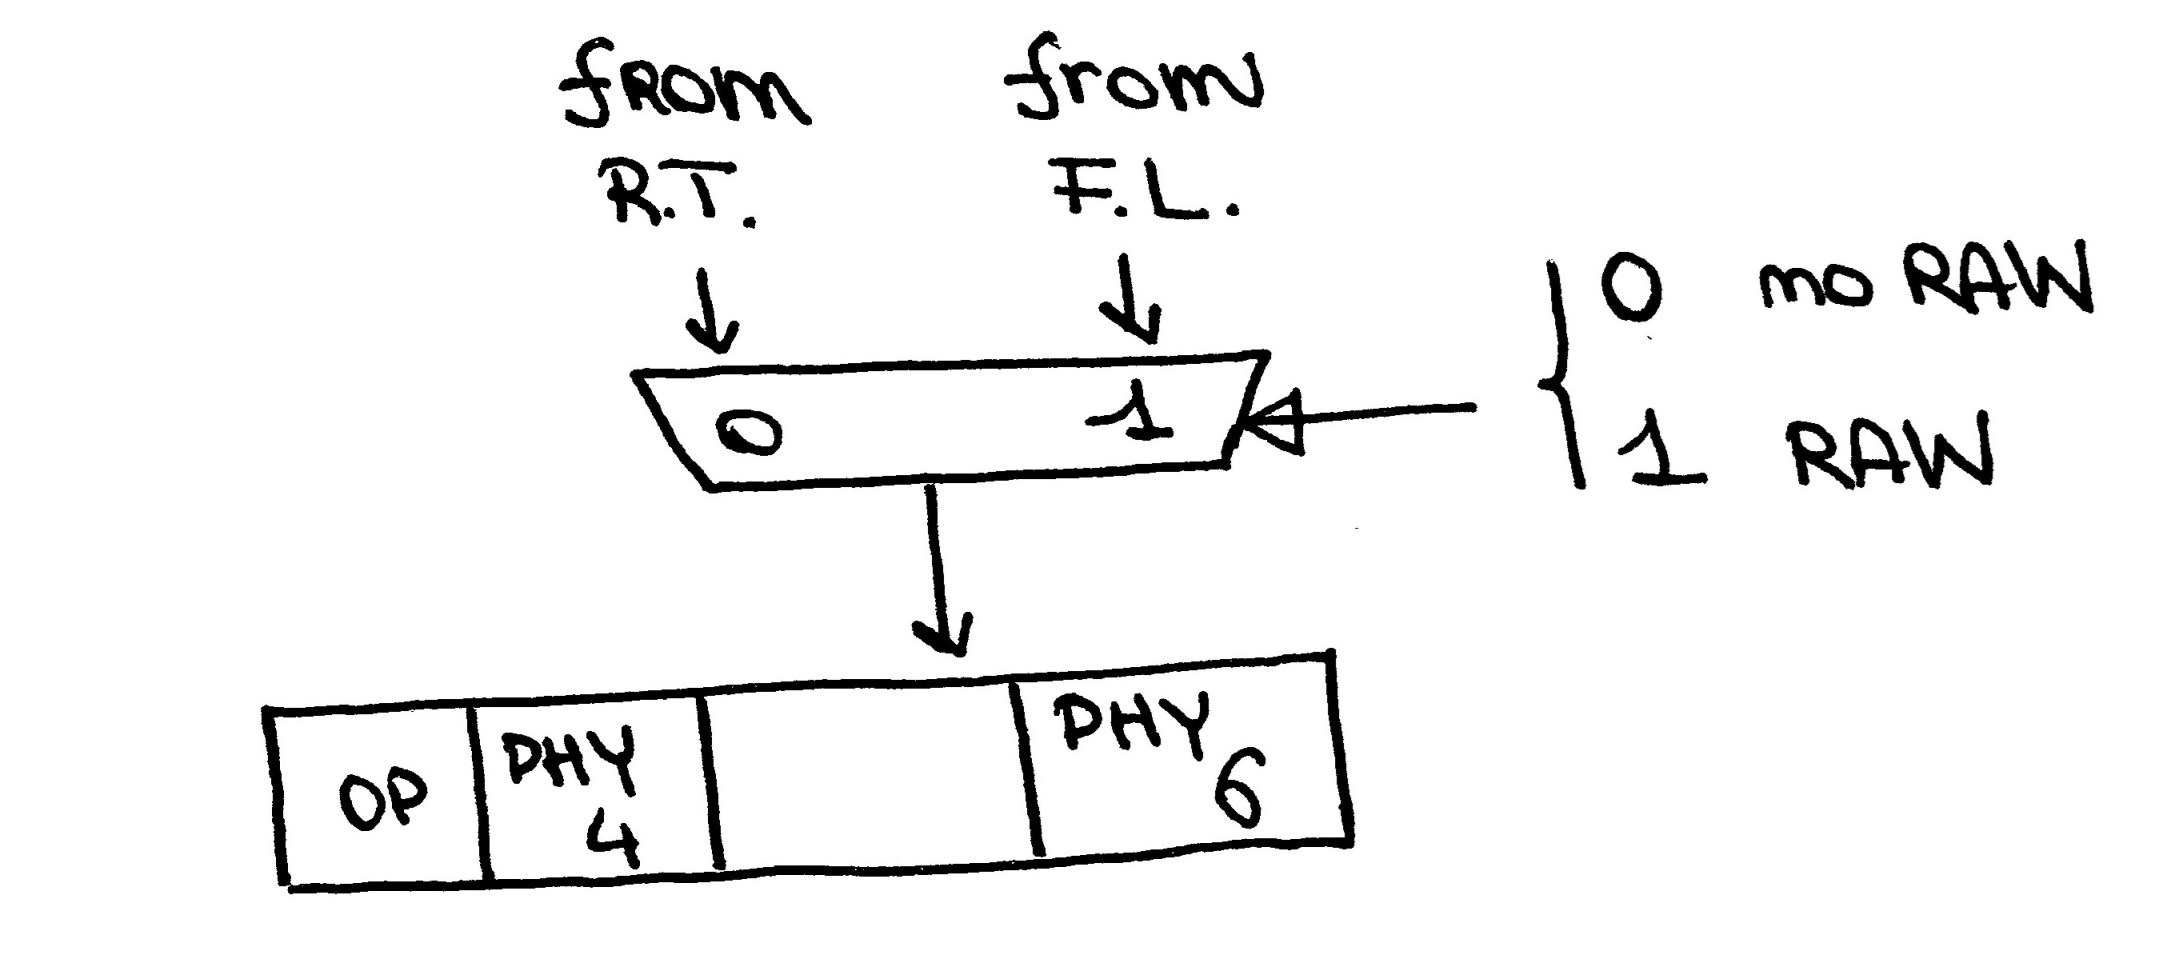
\includegraphics[width=0.7\linewidth]{img/img3/27}
\end{center}

Of course it has to been done for all other source registers, so for a simple 2-parallel instruction processor implementation cost is not so small.

%%%%%%%%%%%%%%%%%%%%%%%%%%%%%%%%%%%%%%%%%%%%%%%%%%%%%%%%%%%%%%%%%%%%%%%%%%%%%%%%
%%%%%%%%%%%%%%%%%%%%%%%%%%%%%%%%%%%%%%%%%%%%%%%%%%%%%%%%%%%%%%%%%%%%%%%%%%%%%%%%
%%%%%%%%%%%%%%%%%%%%%%%%%%%%%%%%%%%%%%%%%%%%%%%%%%%%%%%%%%%%%%%%%%%%%%%%%%%%%%%%

\subsection{Reordering buffer (ROB)}
In out of order processor execution order may be different from the one intended by the programmer. In many cases it is allowed, thanks to register renaming we can delete many conflicts having more freedom in that. However in the last step, results have to be stored in the exact order intended by the programmer. By resuming the last example:

\begin{verbatim}
i1  R1 = R2/R3
i2  R4 = R1+R5    RAW with I1
i3  R5=R6+R7    WAR with I2
i4  R1=R8+R9    WAW with I1
\end{verbatim}

I1 takes much ore time than I4, if I1 and I4 are issued and executed in parallel we can expect I4 to be finished much before I1. If at that time we commit the result of I4 in the logical register, we have changes the semantic of the program (it's only allowed to write I4 result in the corresponding physical register). In order to perform this reordering we need:
\begin{center}
  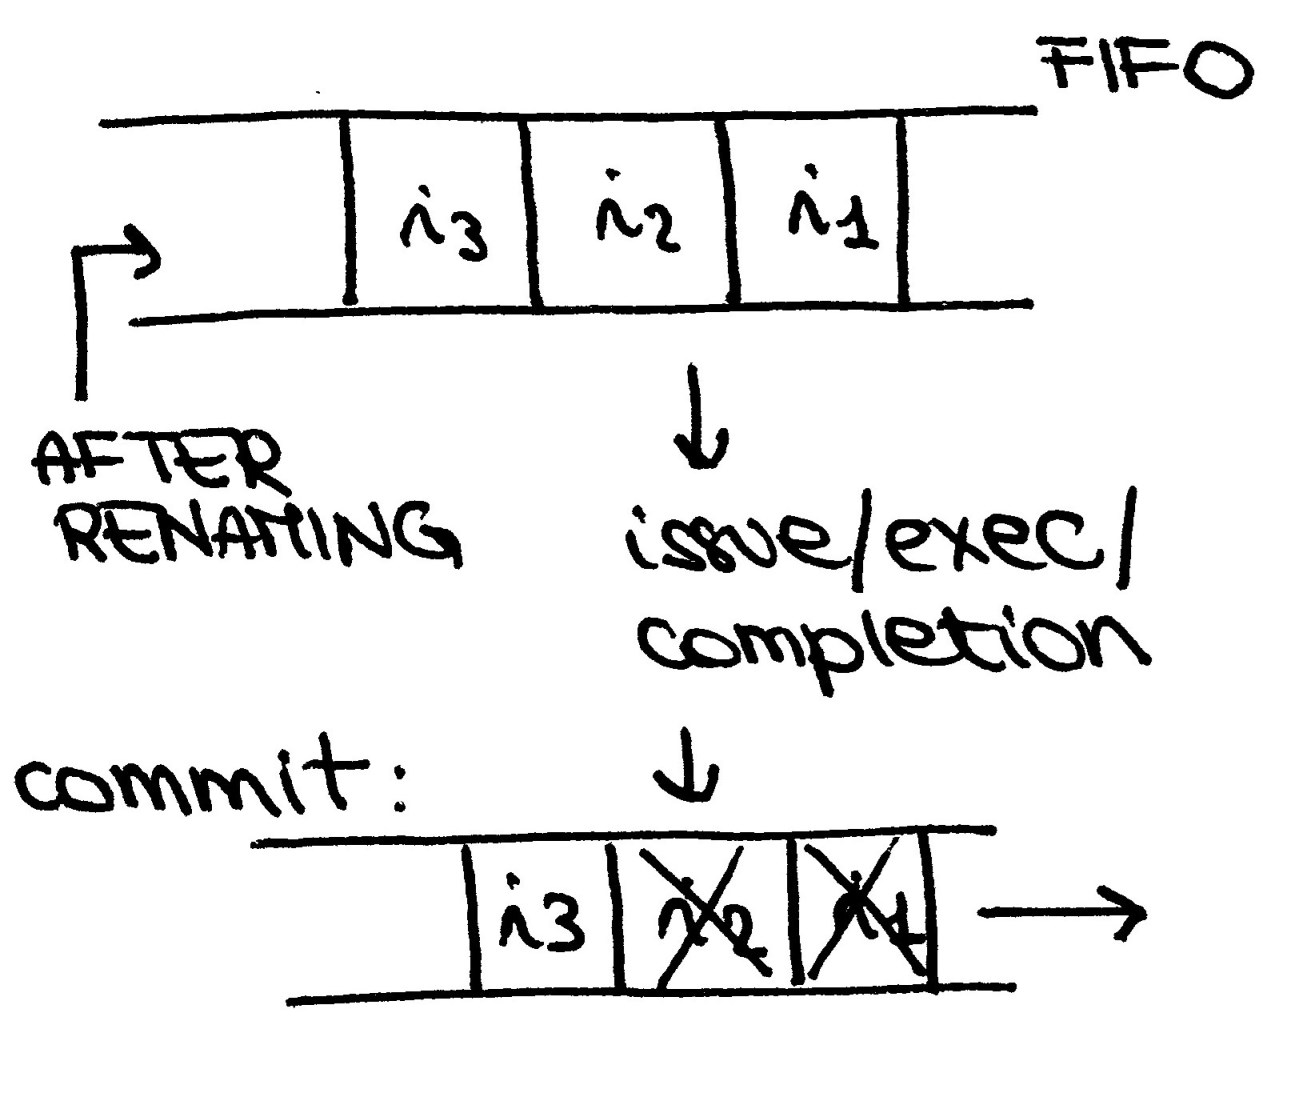
\includegraphics[width=0.5\linewidth]{img/img3/28}
\end{center}

During renaming we insert instructions in a FIFO queue, then we enter the issue /execution/completion stages which works out of order. After them commit operation has to be performed in order by following the queue order. Once I1 has been committed it is flushed away from the queue and proceed to I2 commit (if already available).

\begin{center}
  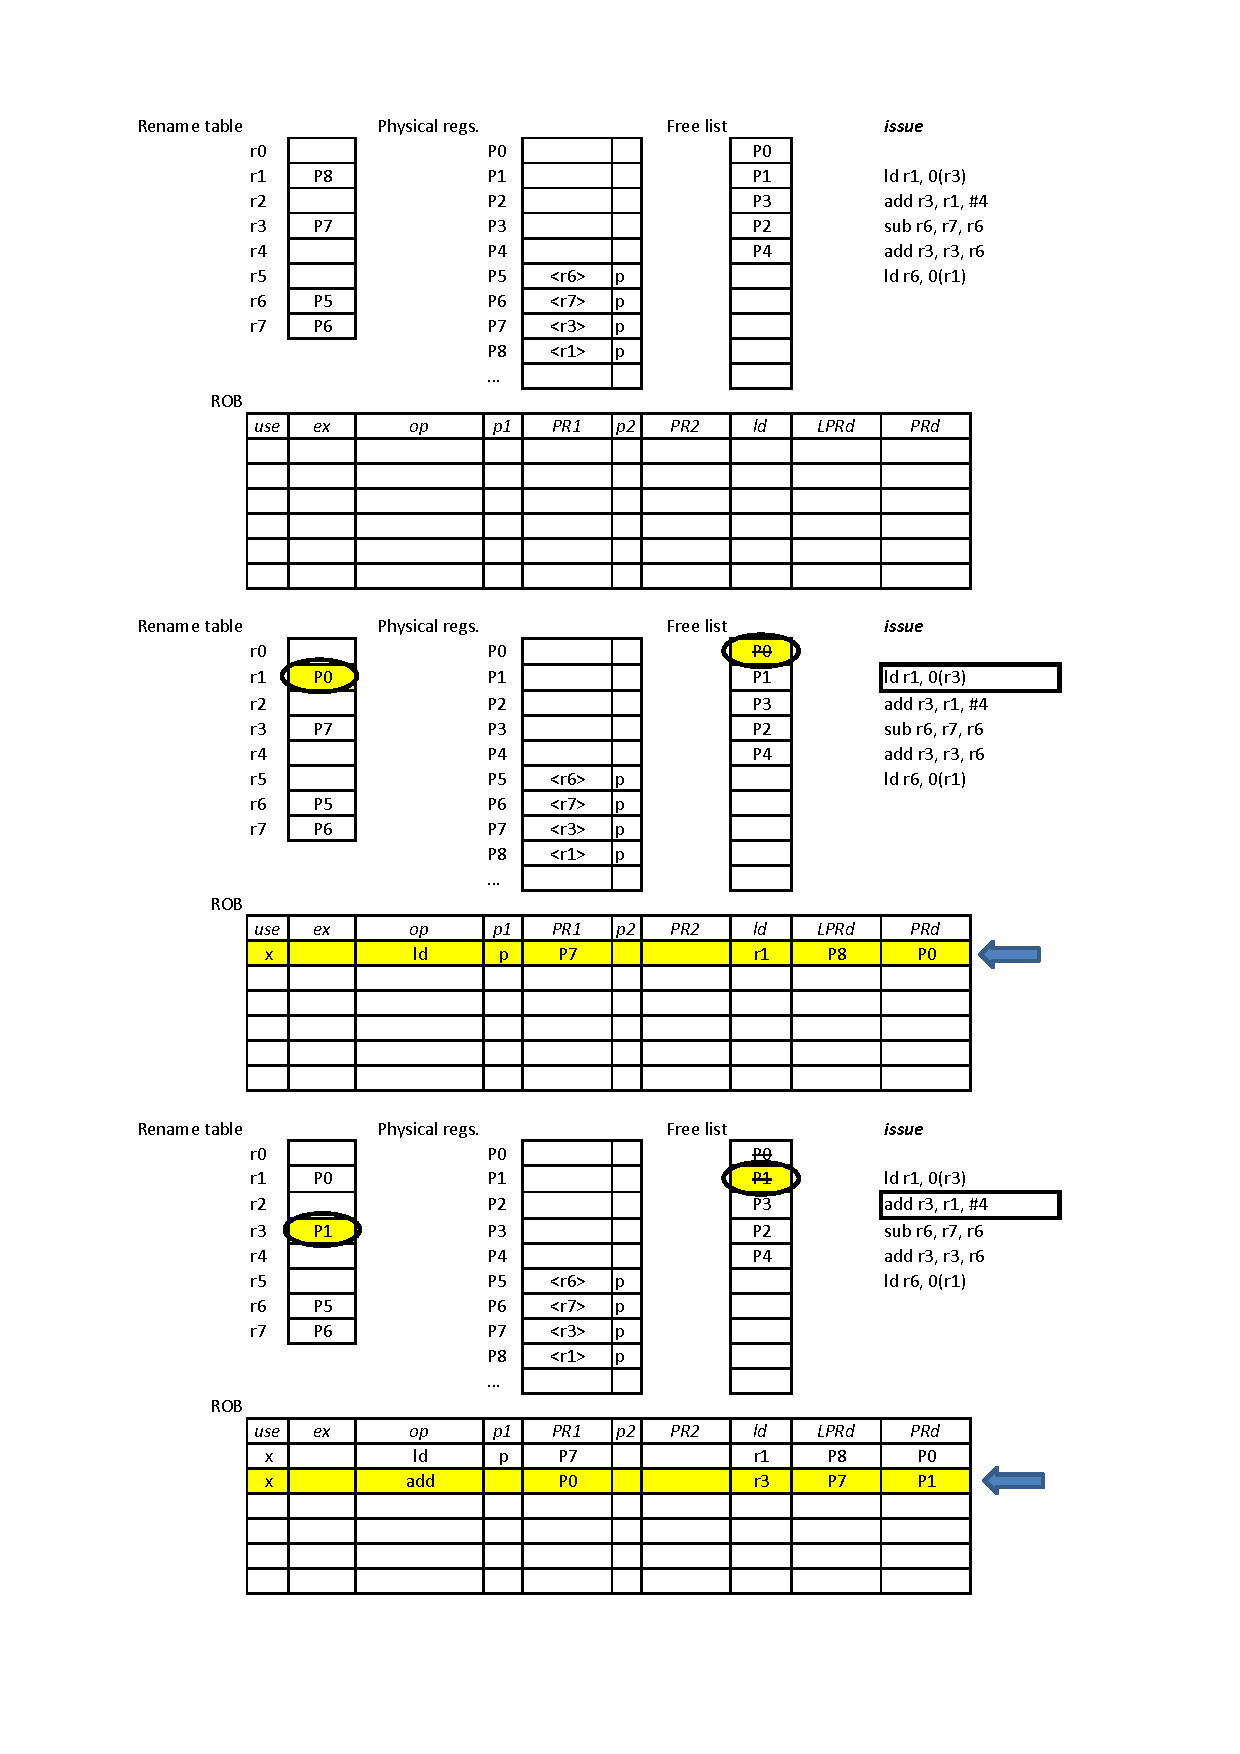
\includegraphics[width=1.1\linewidth]{img/img3/rob_example}
\end{center}


%%%%%%%%%%%%%%%%%%%%%%%%%%%%%%%%%%%%%%%%%%%%%%%%%%%%%%%%%%%%%%%%%%%%%%%%%%%%%%%%
%%%%%%%%%%%%%%%%%%%%%%%%%%%%%%%%%%%%%%%%%%%%%%%%%%%%%%%%%%%%%%%%%%%%%%%%%%%%%%%%
%%%%%%%%%%%%%%%%%%%%%%%%%%%%%%%%%%%%%%%%%%%%%%%%%%%%%%%%%%%%%%%%%%%%%%%%%%%%%%%%

\subsection{Freeing physical registers}

To avoid that free list becomes empty we have to think at a mechanism to put physical registers in free list.

Let's assume R1 to be the logical destination register and P1 the corresponding physical register, in the following instructions we will use P1 (since in all source-like occurrences R1 has been renamed P1) but at a certain point R1 will be reused as destination register: this means that the value written by the first operation in R1 is no more needed, since all the following operations will used the new value of R1. This implies that when R1 is again used as a destination we can free P1.
However this condition is not sufficient since from the programmer point of view it works properly, but due to pipelined/out of order, etc. processor there might be some instructions that still need to use R1 as source register. This means that a double check has to be performed, both we have to reach a second R1 assignment both the old value of P1 has became useless since all instructions requiring it have already been exploited (meaning that all instructions between two assignments have already reached the read stage so P1 is surely in FUs).

This kind of check is quite expensive, a number of solutions has been proposed:

\begin{enumerate}
  \item For each register a counter is allocated, so starting from \verb|R1 <- OP...| we associate to R1 the physical register P1 and in each following instruction where R1 is present as source (like \verb|R2 <- OP R1, ..|) R1 is replaced with P1 and the corresponding counter for R1 is incremented. When this instruction reaches read operand stage (so the actual P1 value is at the beginning of FU) the counter is decremented. At the time we reach a second assignment for R1 (like \verb|R1 <- OP R9, ..|) we have to check counter value: if it is equal to 0 we can free P1, otherwise not since previous value of R1 is still needed somewhere. A counter for each physical register is therefore required.

  \item Wait for the second assignment to be committed for freeing P1, in this way we are sure that the order intended by the programmer is respected.

\end{enumerate}

These two methods are different, 1) is more efficient in term of time but is more expensive, 2) is less expensive but required more time.

%%%%%%%%%%%%%%%%%%%%%%%%%%%%%%%%%%%%%%%%%%%%%%%%%%%%%%%%%%%%%%%%%%%%%%%%%%%%%%%%
%%%%%%%%%%%%%%%%%%%%%%%%%%%%%%%%%%%%%%%%%%%%%%%%%%%%%%%%%%%%%%%%%%%%%%%%%%%%%%%%
%%%%%%%%%%%%%%%%%%%%%%%%%%%%%%%%%%%%%%%%%%%%%%%%%%%%%%%%%%%%%%%%%%%%%%%%%%%%%%%%

\section{Scoreboard data structures}

\subparagraph{Issuing}
Interested fields are:
\begin{itemize}
\item P1,P2: say if operands source data are available.
\item LD: logical destination register.
\item PRd: physical register associated to LD
\item LPRd= previous physical register associated to LD, it is required so we can free the previous physical register.
\end{itemize}


We should take one instruction at the time sequentially, but since our architecture is 2-way parallel we should take two instructions at the same time. In the first step we will issue \verb|ld r1, 0(r3)|, then we perform the issue of second instruction (\# second set of tables), for this second one as source destination we have to indicate the physical reg for r1 which is P0 (rename table), however it is still not available (p1 is not set). Same thing occurs for the following instructions. While we are proceeding in issuing, we are consuming registers from the free list (we almost have no more free regs). To perform all these things in parallel, it is not just sufficient have multiple ports for the memories data but we also should be able to perform all the required tests.

\subparagraph{Execution and commit}
Starting again from the first instruction, the only source operand we have is already available, so we can execute the first instruction At the time we commit the first operation, we take the name of previously physical register associated to r1 which is P8, so we can insert P8 in the free list since the value previously stored in P8 is no more needed and no more instructions in the pipeline need that value (it is in order execution so all previous instructions having r1 as source have already been completed). Proceeding with the following instructions we also need to update the p1 and p2 fields in the ROB table to say that P1 is present.

\begin{center}
  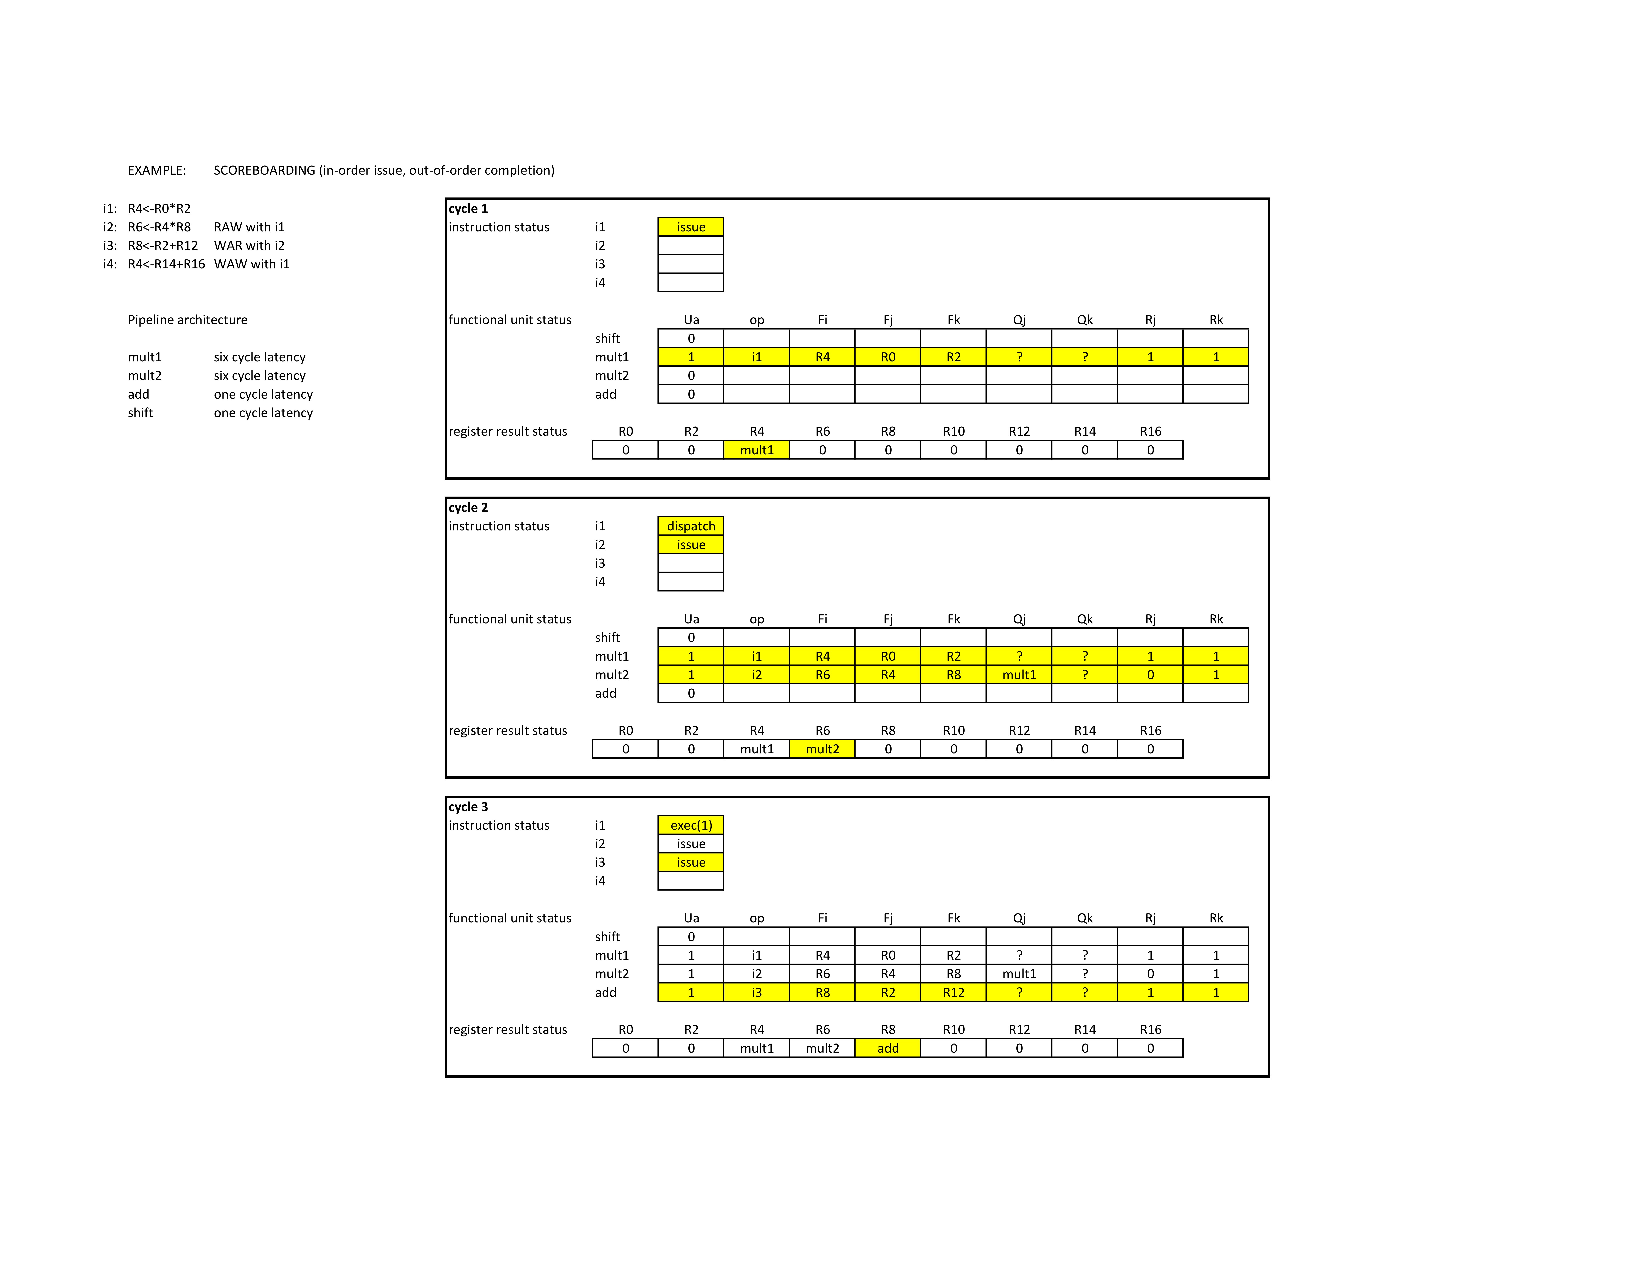
\includegraphics[width=1.0\linewidth]{img/img3/score1}
\end{center}
\begin{center}
  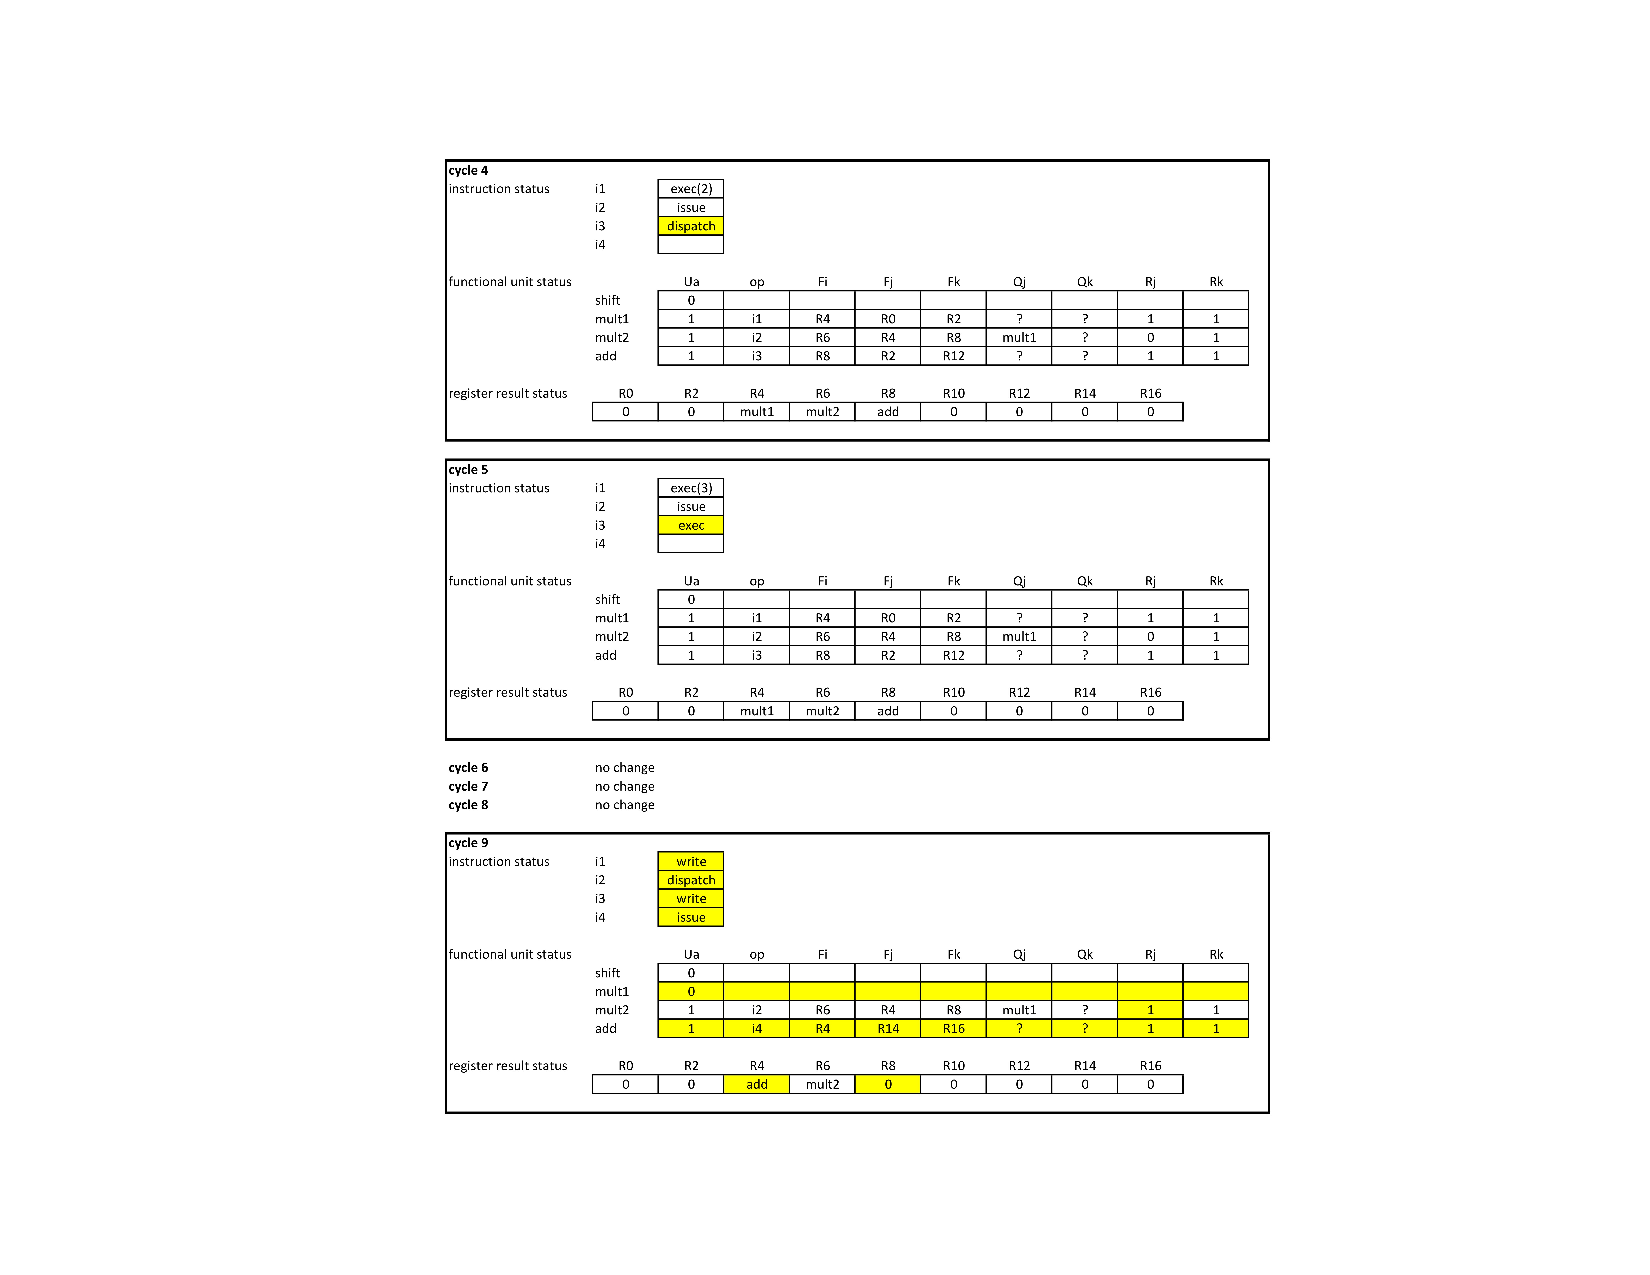
\includegraphics[width=1.0\linewidth]{img/img3/score2}
\end{center}

%%%%%%%%%%%%%%%%%%%%%%%%%%%%%%%%%%%%%%%%%%%%%%%%%%%%%%%%%%%%%%%%%%%%%%%%%%%%%%%%
%%%%%%%%%%%%%%%%%%%%%%%%%%%%%%%%%%%%%%%%%%%%%%%%%%%%%%%%%%%%%%%%%%%%%%%%%%%%%%%%
%%%%%%%%%%%%%%%%%%%%%%%%%%%%%%%%%%%%%%%%%%%%%%%%%%%%%%%%%%%%%%%%%%%%%%%%%%%%%%%%

\section{Memory dependencies}
So far when talking about data dependencies only instructions regarding registers have been taken into account. However similar problems occur when handling data from a memory. Let's consider store (st) and load (ld) operations:

\begin{verbatim}
st  r1, (r2)  // content of register r1 moved in the location pointed by r2
ld r3, (r4)   // read data from location pointed by r4 and put into r1
\end{verbatim}

A data dependency between this two instructions occurs when $r2 = r4$ so it results in a RAW conflict. If this is the case the order of execution cannot be changed, meaning that if our processor is out of order it has to detect and manage this situation, since this kind of conflict cannot be detected at compiler time.
In addition to that the execution of instructions is based on speculation especially for out of order processor (just commit stage is performed strictly in the order intended by the programmer). To avoid these problems we may use an additional data structure, called \textbf{store buffer} inserted between register file and data memory (i.e. data cache). Speculation allows to do everything we want except the final write on data cache, so we employ the store buffer in the middle.
\begin{center}
  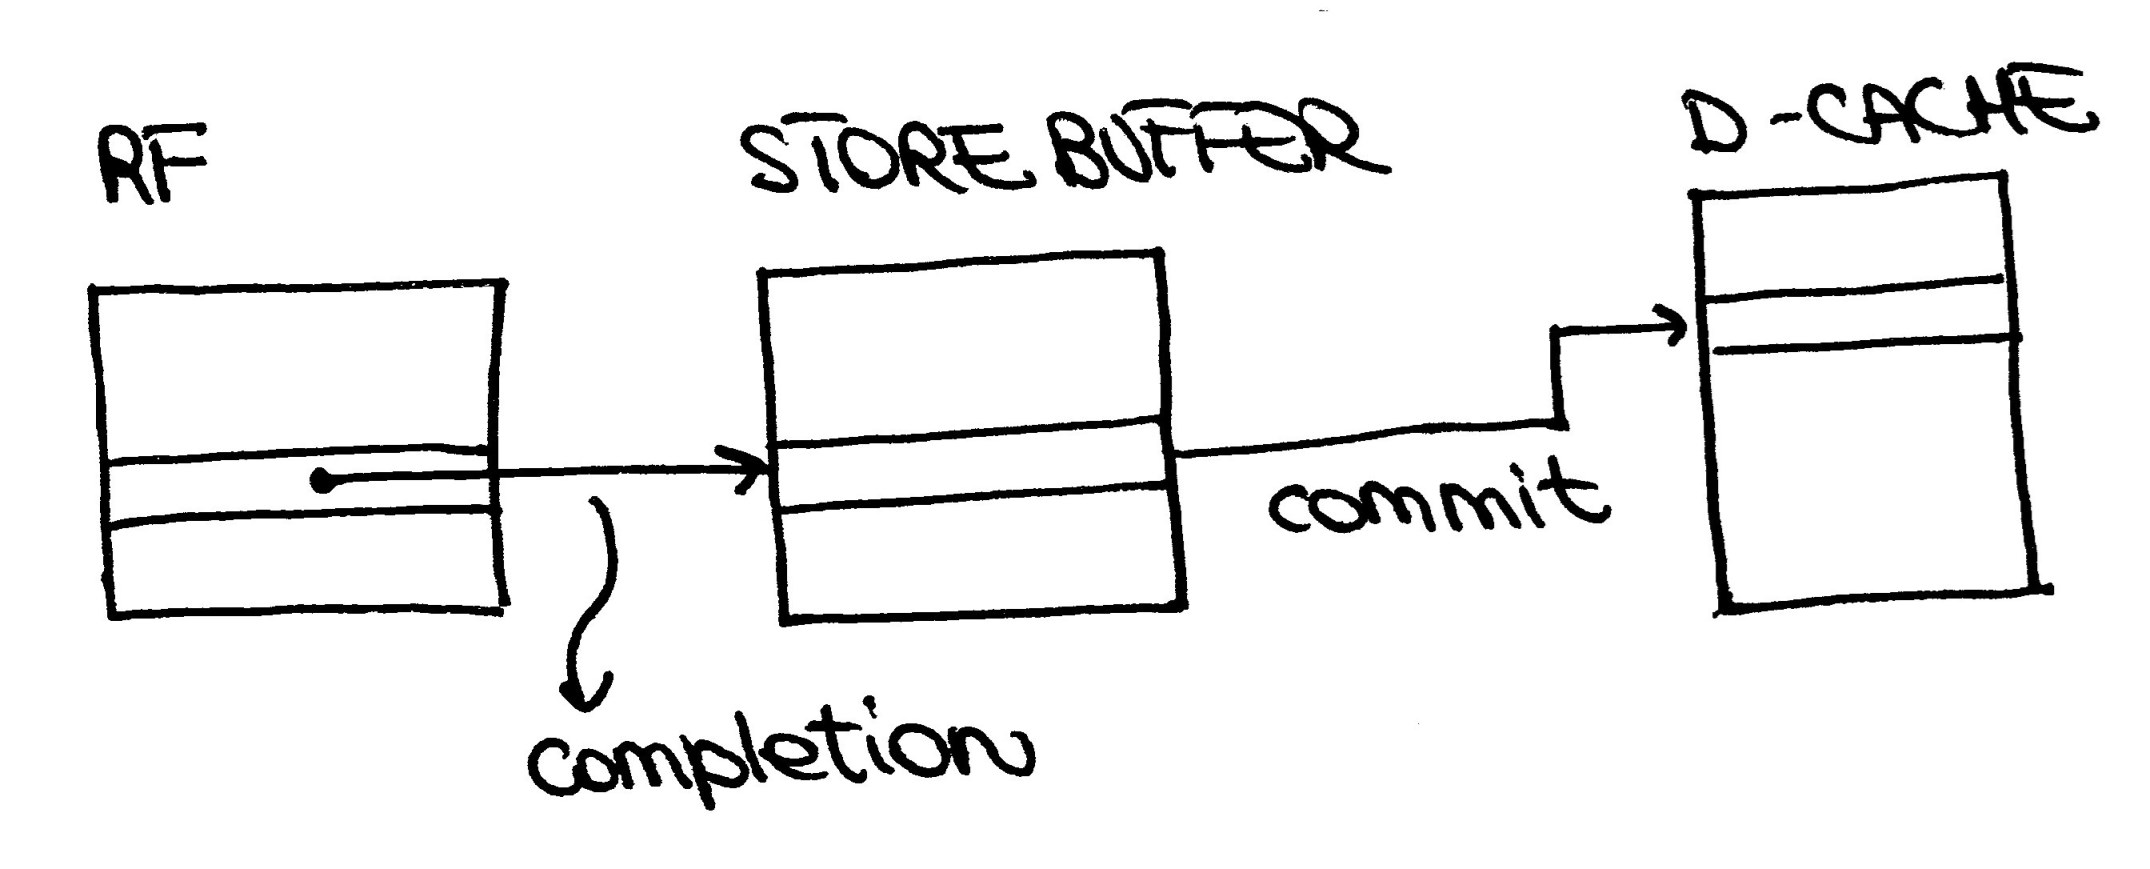
\includegraphics[width=0.7\linewidth]{img/img3/30}
\end{center}

In this way we are able to handle writing operations, but regard reading we have to take the data from D-cache or store buffer? Usually these two works in parallel and both of them are actually cache memories (where each location has valid, tag and data fields).
\begin{center}
  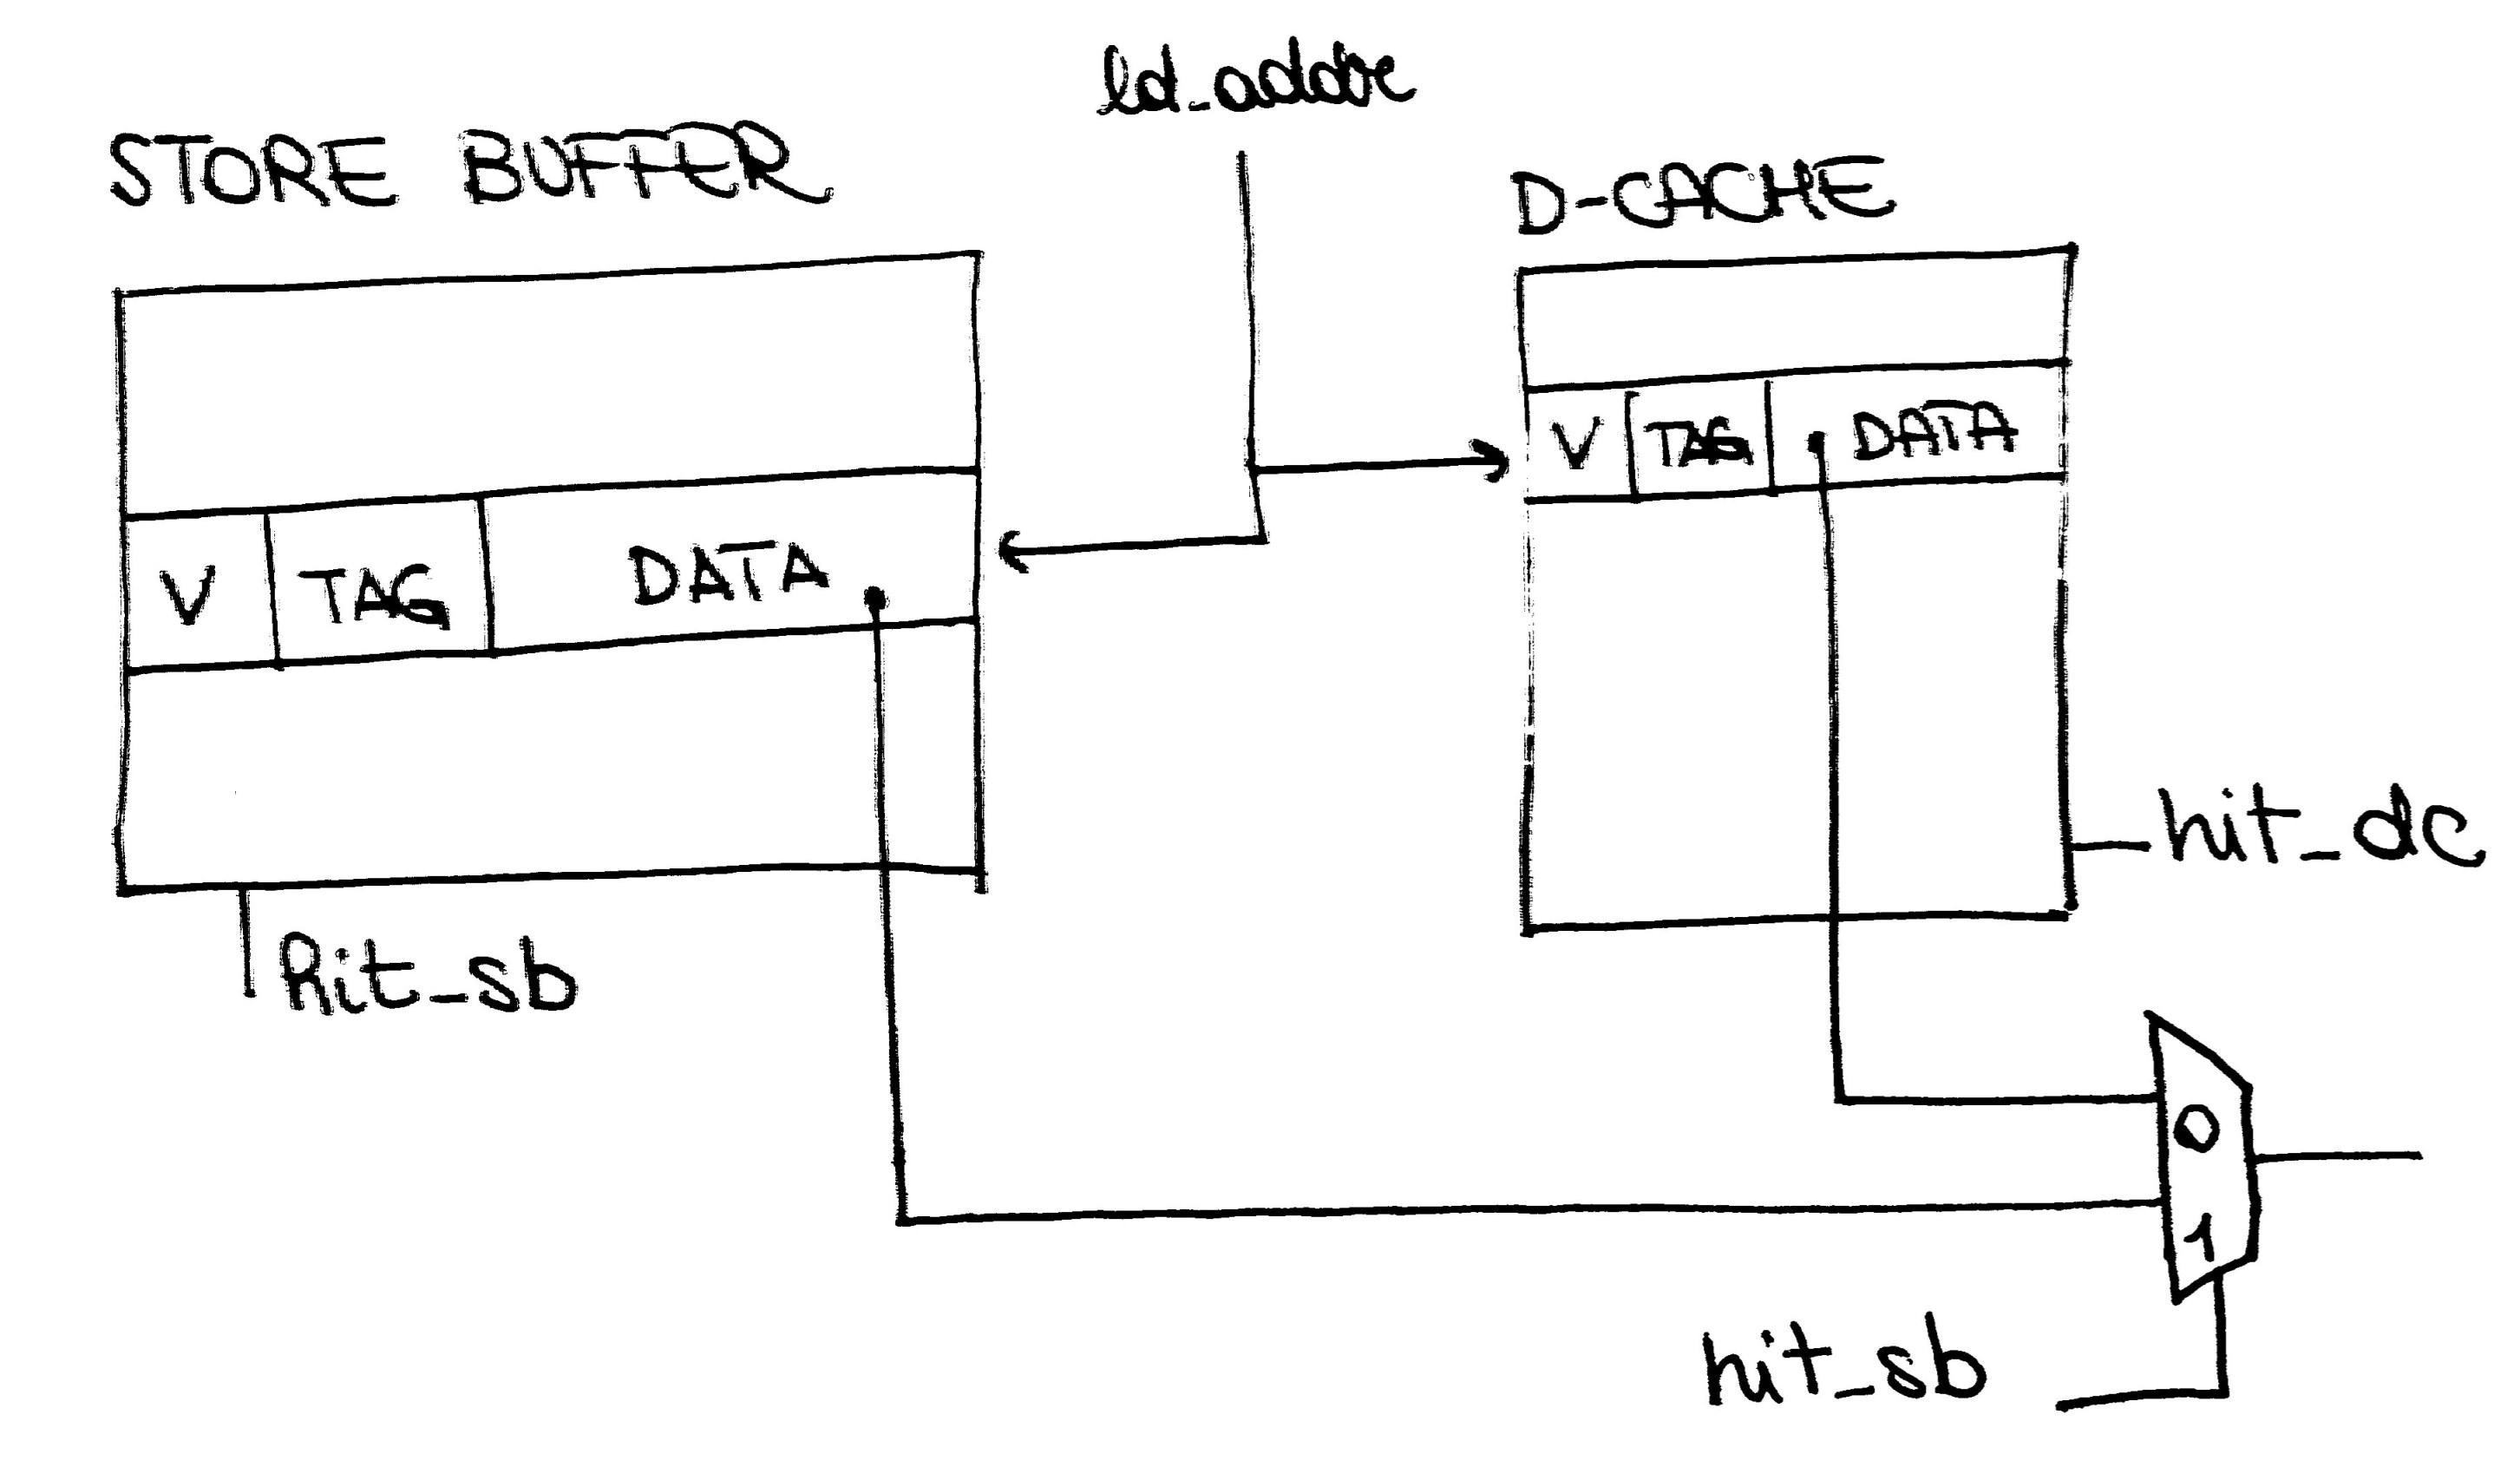
\includegraphics[width=0.7\linewidth]{img/img3/31}
\end{center}
When performing a load instruction, the ld address is applied to both memories in parallel, if the data is currently stored in the store buffer we will take from it, otherwise it means that the data we are looking for will be taken from data-cache (store buffer has a higher priority with respect to D-cache), $h$ is the hit bit. Store buffer is an additional layer of caching, thanks to it we could be allow to change the order of load/store instructions. To handle this new scenario some solutions may be exploited:

\begin{itemize}
  \item \textbf{Conservative out of order execution of load}

  It is allowed for sure if $r4 \neq r2$ so just by comparing the content of these two registers if they are different we can accept the change of order between load and store instructions.  Since comparing two registers may be expensive, we limit comparison to the LSB part of them (16 LSB instead of total 32 bits). If 16 LSB are different, no problem and we can change the order, if they are equal we avoid changing the change of order (although it may happen that the two MSB parts are different). In this approach the change of order is permitted only if we are sure that the two register content is different.

  \item \textbf{Speculative out of order approach}
  We guess that $r4 \neq r2$ so load is possibly executed before store. Later we check if our initial assumption was correct or not, if yes we proceed normally, instead if we discover that $r4=r2$ we have to discharge the two instructions and all subsequent instructions in the pipeline. This may result in a big penalty, like in the branch.

  \item \textbf{Dynamic prediction}
  Like for branch instruction we have a mechanism that dynamically detects data dependencies. At the first occurrence of load and store we make a guess, when we finally know if $r4=r2$ we insert in a binary table the comparison result, so at the next occurrence of these two instructions we may have a better prediction. Just in the first occurrence the guess is random, for the next we have a more confident prediction.

\end{itemize}

\section{Tricks in VLIW architectures}

In this last part some new techniques typical of VLIW processors will be presented. In this kind of architecture there are some troubles regarding branches since from the compiler point of view is difficult to know if a certain branch will be taken or not, so it doesn't know which instructions can be performed in parallel

\subsection{Branch predication}
It is completely different from branch prediction (which exploits the most probable direction for a branch), in this new approach instructions coming from both branches are executed in parallel, there are no mechanisms that try to guess the branch directions, only at the end, before commit step, we decide which branch has to be taken (ALAP approach).

After instruction 3 there are two possible flows so instructions 4...9 are all performed in parallel (usually 4,5,6 have no data dependence with 7,8,9). While performing all this instructions they are also associated to a predicate register, which is 0 or 1 depending on the fact that a certain instruction belongs to left or right flow.

Typically a certain instruction is linked to a certain register, meaning that $<Pi> \leftrightarrow $ instruction i; $Pj Pk = relation$ indicates that the update is always performed, $<Pi> Pj Pk =relation$ means that the update of $P_j$ and $P_k$ is performed only if $Pi$ is true.

\subparagraph{Example}

\begin{verbatim}
if (a && b)
    j=j+1;
else {
    if(c)
        k++;
    else
        k--;
    m=k*5;
}
i= i+1;
\end{verbatim}

Possible situations:

\begin{center}
  \begin{tabular}{|c|l|}
    \hline
    Condition& Instruction\\
    \hline
    if(a != 0 and b !=0)&         \verb|ADI R2, R2, \#1| (immediate sum)\\
    if not(a != 0 and b !=0) and c!=0&    \verb|ADI R4, R4, \#1|\\
    if not (a != 0 and b !=0) and c=0&    \verb|SBI R4, R4, \#1|\\
    if not (a != 0 and b !=0)&        \verb|MPI R5, R4, \#5|\\
    -&                    \verb|ADI R6, R6, \#1|\\
    \hline
  \end{tabular}
\end{center}

The compiler can identify all this conditions, for each condition a certain instruction to be performed is associated. The idea is to associate at each of this condition a predicate register:

\begin{verbatim}
P1, P2 = EQ(R0, \#0)
<P2> P1, P3= EQ (R1, \#0)  -> only if P2 is true this writing is performed
<P3> ADI R2, R2, \#1
<P1> P4, P5= NEQ(R3, \#0) (c!=0, only if P1 is correct)
<P4> ADI R4, R4, \#1       (c!=0 so P4 is true)
<P5> SBI R4, R4, \#1      (c=0 so P5 is true (and P4 is false))
<P1> MPI R5, R4, \#5
   ADI R6, R6, \#1
\end{verbatim}
so P3 is true iff (a != 0 and b !=0) so depending on P3 we can execute the first immediate sum.

\begin{center}
  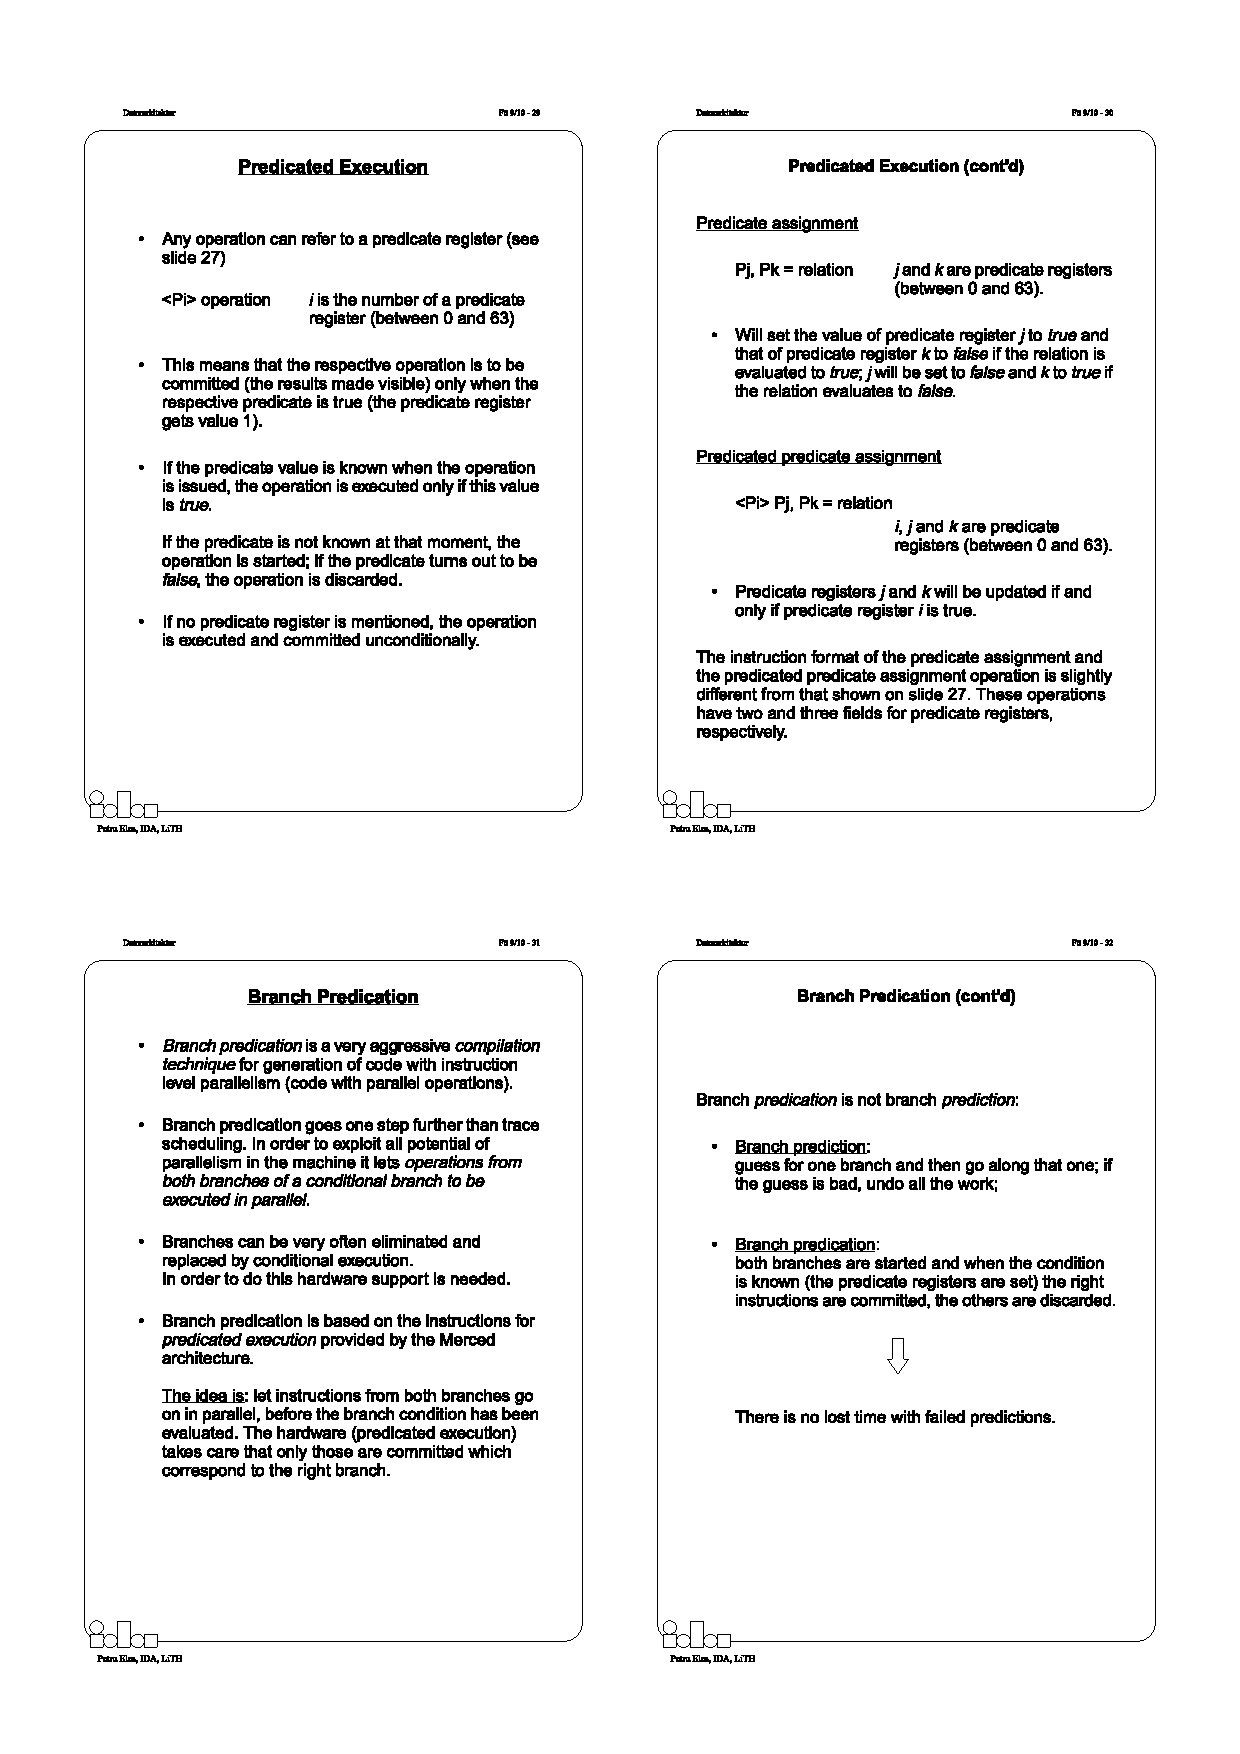
\includegraphics[width=1.1\linewidth]{img/img3/predication}
\end{center}

\begin{center}
  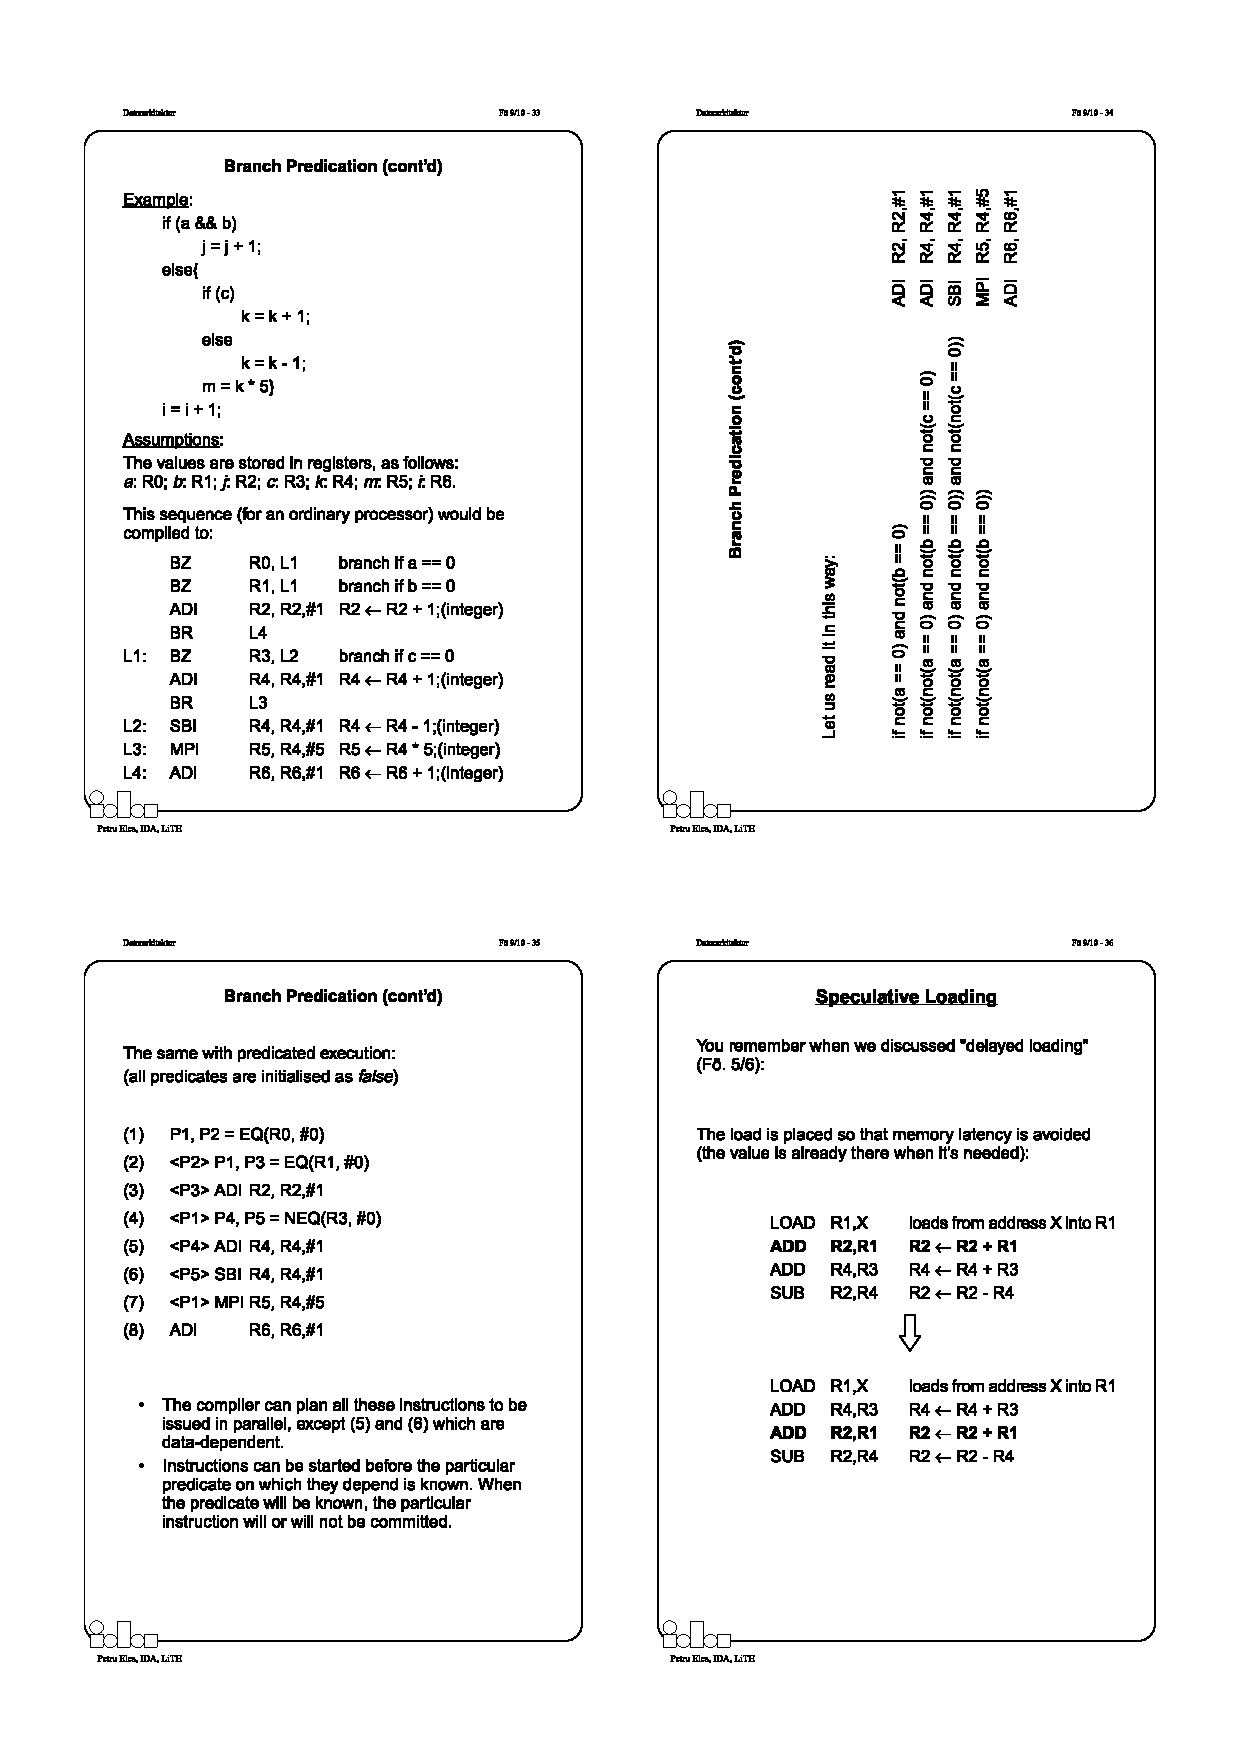
\includegraphics[width=1.1\linewidth]{img/img3/predication2}
\end{center}

\subsection{Software technique to increase parallelism}
To increase further the instruction level parallelism the compiler can:

\begin{itemize}
  \item \textbf{Loop unrolling}: compiler has the chance to identify loops and modify the arrangement of the code with the purpose to increase the degree of parallelism.
  \subparagraph{Example}
  \begin{verbatim}
  for(i=0; i< n; i++) {
      add
      add
  }
  \end{verbatim}
  The potential parallelism inside the single operation is only equal to two, so if our VLIW have 4 FU so that 4 additions can be performed at the same time, using this approach we are exploiting only 50 \% of available resources. The loop therefore can be unrolled by halfing the number of iterations
  \begin{verbatim}
  for(i=0; i< n/2; i++) {
      add1
      add2
        add3
        add4
  }
  \end{verbatim}

  Providing that there are no data dependencies, in this way we can reach 100 \% of resources usage.

  \item \textbf{Trace scheduling}:
  \begin{center}
    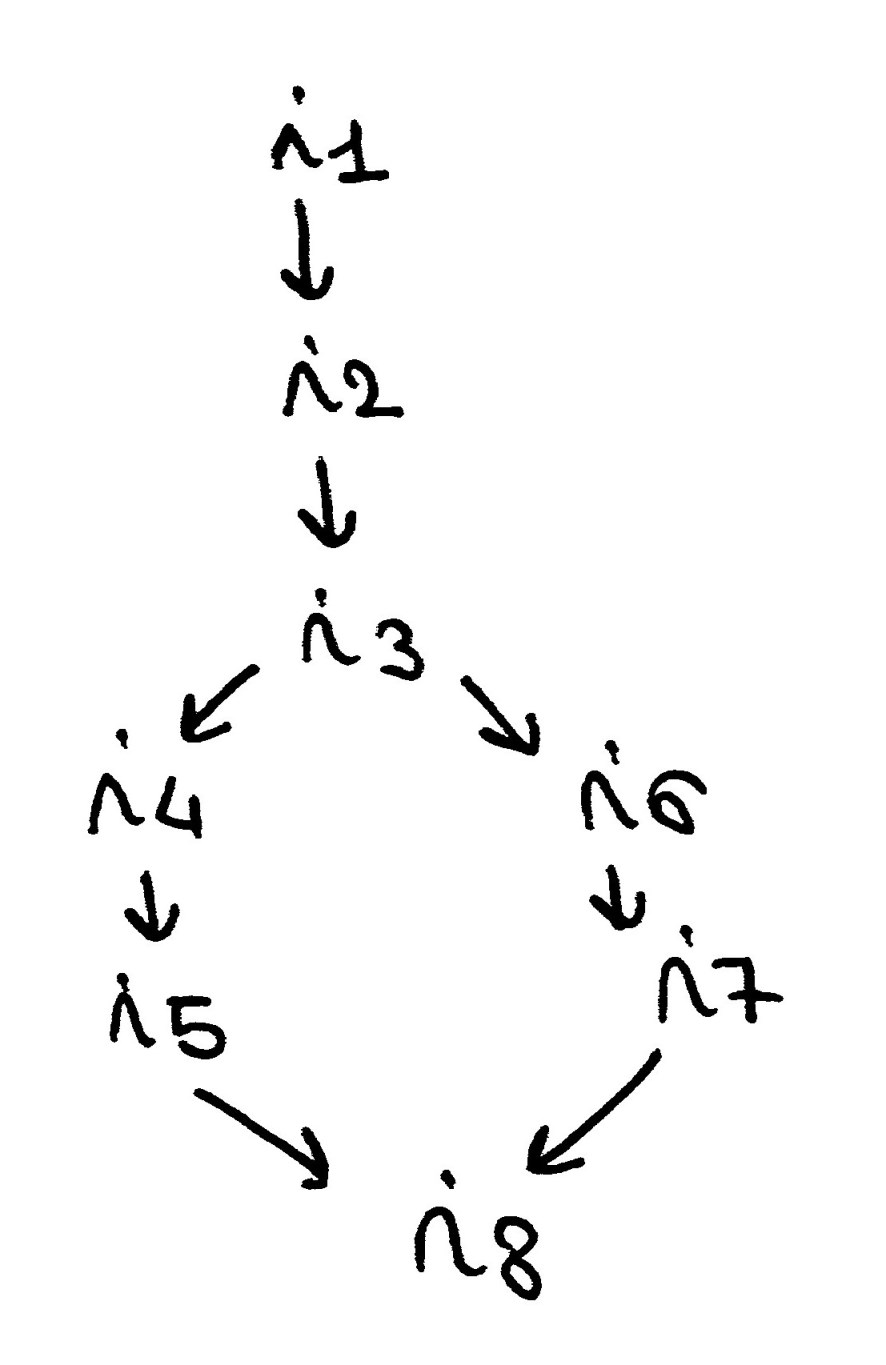
\includegraphics[width=0.2\linewidth]{img/img3/32}
  \end{center}

  In this example i3 is a branch so by profiling the compiler may know which is the more
  probable path. If this is the case, all instructions coming from the most
  probable path scheduling they are arranged to be performed as much as possible
  in parallel, so we extend the set of instructions to be performed in parallel
  beyond the boundary of branches, obtaining the degree of parallelism is better. In
  this way the execution is out of order and it is determined by the compiler. \\

  If the prediction made from the compiler is wrong, we have to discharged the wrong
  operations, so we have to insert some more instructions to be able to perform
  the right operations and make some compensations. For a compiler this compensation code is not difficult to be
  determined (while for dynamic approach is much more complex).

\end{itemize}
